\documentclass[a4paper,10pt]{book}
\usepackage[english]{babel}
\usepackage[T1]{fontenc}
\usepackage[utf8]{inputenc}
\usepackage{lmodern}
\usepackage{geometry}
\geometry{verbose,tmargin=3cm,bmargin=3cm,lmargin=2cm,rmargin=2cm}
\usepackage{fancyhdr}
\pagestyle{fancy}
\usepackage{amsthm}
\usepackage{amsmath}
\usepackage{array,multirow}
\usepackage{amsfonts}
\usepackage{amssymb}
\usepackage{mathtools}
\usepackage[authoryear]{natbib}
\usepackage{algorithm}
\usepackage{algpseudocode}
\usepackage[hyphens]{url}
\usepackage{color}
\usepackage{graphicx}
\usepackage[table]{xcolor}
\usepackage{booktabs}
\usepackage{import}
\usepackage{bm}
\usepackage{listings}
\usepackage{dirtree}
\graphicspath{{Figures/}}
\usepackage{minted}
\usepackage{float}
\usepackage{subfig}
\usepackage{tikz}
\usetikzlibrary{trees}
\usepackage{framed}
\usepackage{tcolorbox}
\usepackage[colorlinks=true,linkcolor=red]{hyperref}

\makeatletter
\tcbuselibrary{minted,skins}
\newtcblisting{bashcode}{
	listing engine=minted,
	colback=bashcodebg,
	colframe=black!70,
	listing only,
	minted style=bw,
	minted language=bash,
	minted options={texcl=true},
	left=1mm,
}
\definecolor{bashcodebg}{rgb}{0.85,0.85,0.85}
\makeatother

\bibliographystyle{apalike2}

\floatstyle{plain}
\newfloat{code}{Ht!}{loc}[chapter]
\floatname{code}{Code}

\begin{document}

\newcommand \xmltag[1] {\textcolor{blue}{\texttt{<#1>}}}
\newcommand \xmlfield[2] {\item[-] \xmltag{#1} #2 \xmltag{/#1}}

\tikzstyle{every node}=[draw=black,thick,anchor=west]
\tikzstyle{selected}=[draw=red,fill=red!30]
\tikzstyle{optional}=[dashed,fill=gray!50]

\newcommand{\surname}{RAFFO}
\newcommand{\initials}{AVL}
\newcommand{\reportnumber}{1}
\newcommand{\reportversion}{1.0}
\newcommand{\reporttitle}{ProVANT Simulator User Guide}
\newcommand{\autor}{Arthur Viana Lara}
\newcommand{\translator}{Daniel Leite Ribeiro}
\newcommand{\version}{1.0}

\newcommand{\macroheader}[4]{MACRO/#1--\the\year /#2/#3+Version-#4}


\lfoot{\noindent \macroheader{\surname}{\initials}{\reportnumber}{\reportversion}}


\cfoot{}


\rhead{\noindent 
\includegraphics[width=0.15\textwidth]{report_template/macro_inline}}


\rfoot{\thepage}


\lhead{\leftmark}

\thispagestyle{empty}

\noindent \begin{center}
\textbf{}%
\begin{minipage}[t]{1\columnwidth}%
\noindent \begin{center}
\textbf{}%
\begin{minipage}[c]{0.3\columnwidth}%
\noindent \begin{flushleft}
\includegraphics[width=1\textwidth]{report_template/macro_inline_name}
\par\end{flushleft}%
\end{minipage}\textbf{}%
\begin{minipage}[b]{0.7\textwidth}%
\noindent \begin{flushright}
\textbf{\macroheader{\surname}{\initials}{\reportnumber}{\reportversion}}
\par\end{flushright}%
\end{minipage}
\par\end{center}%
\end{minipage}
\par\end{center}

\noindent \rule[0.5ex]{1\textwidth}{1pt}

\bigskip{}


\begin{center}
\textbf{\Large{}Universidade Federal de Minas Gerais - UFMG}
\par\end{center}{\Large \par}

\begin{center}
\textbf{\large{}}
\par\end{center}{\large \par}

\vspace{6cm}


\begin{center}
{\LARGE{}\reporttitle}
\par\end{center}{\LARGE \par}

\vfill{}


%\textit{\emph{\large{}Student registration number: \registrationnumber}}{\large \par}

\textit{\emph{\large{}Autor: \autor}}{\large \par}

%\textit{\emph{\large{}Advisor: \advisorname}}{\large \par}

\textit{\emph{\large{}Versão: \version}}{\large \par}

\vspace{1cm}


\begin{flushright}
\textit{\emph{\today}}
\par\end{flushright}

\pagebreak{}


\chapter*{Abstract}~

The purpose of this guide is to describe the required procedures for using ProVANT Simulator. Its covers from the installation process to performing tests on control strategies via simulation. The text is organized as follows:

\begin{enumerate}
	\item The first section presents the context in which this simulation environment is inserted, and also a brief introduction on unmanned aerial vehicles (UAVs);
	\item The second section presents the steps required for the installation of ProVANT's simulatioin environment;
	\item The third section describes the simulation environment's workflow, detailing each feature of the GUI, such as choosing scenario, model, control strategy and airship.
	\item The fourth chapter is the most important for the user. It describes the procedures for implementing new control strategies in the simulation environment;
	\item Appendix A explains the file structure behind the UAV models used. In this section is presented the main information about kinematic modelling and about importing files from CAD software into the platform Gazebo;
	\item Appendix B describes the plugins used in the simulation environment;
	\item Appendices C end D describe the files {\tt CMakeLists.txt} and {\tt package.xml}, respectively.
\end{enumerate}

\tableofcontents
\listoffigures
\listoftables
\listof{code}{List of Code Snippets}

\chapter{Introdução}

Veículos aéreos não tripulados (VANTs) são aeronaves equipadas com sistemas embarcados, sensores e atuadores que permitem a realização de voos autônomos ou remotamente controlados. Eles são comumente classificados em dois grupos: veículos de asas rotativas, como helicópteros e quadrotores, e veículos de asas fixas, como aviões. 

Há diversas aplicações para VANTs, alguns exemplos são:

\begin{itemize}
	\itemsep0em
	\item Pulverização de culturas;
	\item Condução de rebanhos;
	\item Monitoramento de estradas;
	\item Inspeção da linhas de energia;
	\item Entrega de suprimentos em locais de difícil acesso.
	\end{itemize}
	
O simulador apresentado neste manual está associado ao ProVANT\footnote{provant.eng.ufmg.br}. O ProVANT consiste em uma parceria entre a Universidade Federal de Santa Catarina e a Universidade Federal de Minas Gerais, com o objetivo de realizar pesquisas e desenvolver novas tecnologias para aperfeiçoar o desempenho de VANTs. Neste contexto, atualmente, o ProVANT está focado no desenvolvimento de VANTs Tilt-rotor.  O Tilt-rotor é uma aeronave que possui configuração híbrida, portanto apresenta as principais vantagens das aeronaves de asa fixa e de asa rotativa, como por exemplo consumo reduzido de energia em voos de cruzeiro e decolagem e pouso na vertical. Ele pode operar tanto em ambientes fechados quanto abertos.

Atualmente o ProVANT possui três tipos de linhas de projeto:
	\begin{enumerate}
		\item Mecânico/Aerodinâmico;
		\item Instrumentação/Eletrônica;
		\item Projeto de estratégias de controle e estimação de estados;
	\end{enumerate}

O projeto Mecânico/Aerodinâmico já conta com 5 versões de VANTs que foram nomeadas como VANT 1.0, 2.0, 2.1, 3.0 e 4.0, as Figuras \ref{vant1}, \ref{vant2}, \ref{vant21}, \ref{vant3} e \ref{vant4} ilustram, respectivamente, essas versões. A Instrumentação/Eletrônica está em estágio avançados, com todos os circuitos eletrônicos desenvolvidos e realizando melhorias nos mesmos. Com relação ao Projeto de estratégias de controle e estimação de estados, no contexto do projeto diversas estratégias de controle foram propostas por alunos de mestrado e doutorado.

Ainda com relação ao Projeto de estratégias de controle e estimação de estados, alguns trabalhos científicos foram desenvolvidos. Em \cite{Donadel2015} controladores baseados nas técnicas \textit{Linear Quadratic Regulator} (LQR), $\mathcal{H}_\infty$ linear e $\mathcal{H}_2/\mathcal{H}_\infty$ linear misto foram desenvolvidos para o VANT 1.0. Com o objetivo de rastreamento de trajetória. Alguns destes controladores foram validados através de voos experimentais. Em \cite{Marcelinol2014} é apresentado uma técnica de controle não-linear baseado em \textit{feedback linearization} com o objetivo de transporte de carga para o VANT 2.0, ainda com o mesmo objetivo, \cite{Richard2016} apresenta o desenvolvimento de um controlador baseado na técnica \textit{Model Preditive Control} (MPC). Em \cite{Brenner2016}, trabalhou-se com o transporte de carga do VANT 2.0, no entanto, abordou-se o problema de seguimento de trajetória do ponto de vista da carga, para o qual foram projetados estimadores de estados robustos. Em \cite{Daniel2016}, desenvolveu-se uma estratégia de controle adaptativo com a finalidade de seguimento de trajetória para o VANT 3.0. 
		
\begin{figure} [H]
		\centering
		\begin{minipage}{.5\textwidth}
			\centering
			\includegraphics[height=3.5cm]{figuras/VANT1}
			\caption{Projeto mecânico VANT 1.0.}
			\label{vant1}
		\end{minipage}%
		\begin{minipage}{.5\textwidth}
			\centering
			\includegraphics[height=3.5cm]{figuras/VANT2}
			\caption{Projeto mecânico VANT 2.0.}
			\label{vant2}
			\end{minipage}
	\end{figure}
					
	\begin{figure} [H]
		\centering
		\begin{minipage}{.5\textwidth}
			\centering
			\includegraphics[height=3.5cm]{figuras/VANT21}
			\caption{Projeto mecânico VANT 2.1.}
			\label{vant21}
		\end{minipage}%
		\begin{minipage}{.5\textwidth}
			\centering
			\includegraphics[height=3.5cm]{figuras/VANT3}
			\caption{Projeto mecânico VANT 3.0.}
			\label{vant3}
		\end{minipage}
	\end{figure}
								
	\begin{figure} [H]
		\centering
		\begin{minipage}{.5\textwidth}
			\centering
			\includegraphics[height=3.5cm]{figuras/VANT4}
			\caption{Projeto mecânico VANT 4.0.}
			\label{vant4}
		\end{minipage}
	\end{figure}

O simulador ProVANT tem o objetivo de ser uma ferramenta confiável e de fácil utilização. O intuito é possibilitar a redução de custos e de tempo necessário para o projeto e validação de estratégias de controle.
\chapter{Installation}

ProVANT Simulator is a simulation environment developed in order to validate and evaluate the performance of control strategies. The simulator version addressed in this guide was develop on top of Gazebo 7, a simulation platform, and ROS (Robot Operating System), a framework for developing robot applications, under the Kinetic distribution. In order to use it, a computer running the \textbf{operating system Ubuntu 16.04} is needed.

ROS offers a programming interface for robotics applications and features repositories with several software modules, and Gazebo is a 3D simulation software under free license, maintained and developed under responsibility of the Open Source Robotics Foundation (OSRF). It's able to simulate the dynamic behavior of rigid, articulated bodies, and includes features such as collision detection and graphical visualization.

This chapter presents the steps required for installation of ProVANT Simulator. It first presents the installation procedures for the platforms used by the simulator, such as Qt5, Git and ROS, and then those for the ProVANT simulation environment.

\section{Installation procedures}

In the steps described here it is assumed that the computer in which the simulator is being installed runs a clean, recently installed copy of Ubuntu 16.04.

\subsection{Installing Git}

She source code for ProVANT simulator is hosted on GitHub. In order to access the source code flies for ProVANT hosted on this GitHub repository, Git must be installed in the user's computer. In case it's not, open a new terminal and run the following commands:

\begin{bashcode}
sudo apt update
sudo apt install git
\end{bashcode}

\subsection{Installing and configuring ROS}

ROS offers a programming interface for robotics applications and several software modules, among which is simulator Gazebo, version 7, used by ProVANT Simulator. This subsection details the instructions needed for installing the ROS Kinetic Kame distribution\footnote{More details and help can be found on \href{wiki.ros.org}{ROS's homepage}}.\\
\bigskip
\bigskip
\bigskip

\textbf{Configure the Ubuntu repositories}\\

Before starting installation, the Ubuntu repositories must be configured to allow \textit{restricted}, \textit{universe} and \textit{multiverse}. Note: Usually, this options are already set upon installation of Ubuntu 16.04. In case they're not, follow the \href{https://help.ubuntu.com/community/Repositories/Ubuntu}{Ubuntu guide} for instructions on doing this.

\textbf{Setup sources.list}\\

The computer must also be set up to accept software from packages.ros.org. To do that, open a new terminal and run the following command:

\begin{bashcode}
sudo sh -c 'echo "deb http://packages.ros.org/ros/ubuntu $(lsb_release -sc) main"
>/etc/apt/sources.list.d/ros-latest.list'
\end{bashcode}

\textbf{Setup access keys for ROS repositories}\\

Run the following command:

\begin{bashcode}
sudo apt-key adv --keyserver hkp://ha.pool.sks-keyservers.net:80 --recv-key 
421C365BD9FF1F717815A3895523BAEEB01FA116
\end{bashcode}

\textbf{Installation}\\

First, make sure the Debian package index is up-to-date:

\begin{bashcode}
sudo apt update
\end{bashcode}

After updating the packages, download the binary files:

\begin{bashcode}
sudo apt install ros-kinetic-desktop-full
\end{bashcode}

\textbf{Initialize rosdep}\\

Before using ROS, rosdep must be initialized. This system installs the system dependencies for the source code to be compiled. It is required in order to run some core components in ROS.

\begin{bashcode}
sudo rosdep init
rosdep update
\end{bashcode}

\textbf{Environment setup}\\

To have the ROS environment variables automatically added to the bash session every time a new shell is launched:

\begin{bashcode}
echo "source /opt/ros/kinetic/setup.bash" >> $HOME/.bashrc
source $HOME/.bashrc
\end{bashcode}

\textbf{Create a ROS workspace}\\

Finally, a ROS workspace must be created. To do that, run the following command sequence:

\begin{bashcode}
mkdir -p $HOME/catkin_ws/src
cd $HOME/catkin_ws/
catkin_make
source $HOME/catkin_ws/devel/setup.bash
echo "source $HOME/catkin_ws/devel/setup.bash" >> $HOME/.bashrc
\end{bashcode}

\subsection{Installing Qt Framework}

In order to appropriately install ProVANT Simulator's graphical setup environment, QtCreator 5 IDE must be installed. To do that, run the following commands:

\small
\begin{bashcode}
cd $HOME/Downloads
wget http://download.qt.io/official_releases/online_installers/qt-unified-linux-x64-online.run
sudo chmod +x qt-unified-linux-x64-online.run
./qt-unified-linux-x64-online.run
\end{bashcode}
\normalsize


\subsection{Dowloading and installing the simulation environment}

The source code for ProVANT Simulator is located in \href{https://github.com/Guiraffo/ProVANT-Simulator}{this GitHub repository}. Since it's currently private, access must be requested from Professor Guilherme Vianna Raffo\footnote{raffo@ufmg.br}.

Once it's been granted, the current version of the simulation environment can be downloaded by cloning the repository into the user's computer:

\begin{bashcode}
cd $HOME/catkin_ws/src
git clone https://github.com/Guiraffo/ProVANT-Simulator.git
\end{bashcode}

Once cloned, the simulation environment can be installed and configured by running the following commands:

\begin{bashcode}
cd $HOME/catkin_ws/src/ProVANT-Simulator
sudo chmod +x install.sh
./install.sh
\end{bashcode}


Provided that all the procedures described above were executed successfully, the user will be ready to proceed to the next chapter, regarding ProVANT Simulator's workflow.
\chapter{Workflow}
\label{workflow}

This chapter presents the features available for ProVANT Simulator's operation through the graphical interface, such as:

\begin{itemize}
\setlength{\itemsep}{1pt}
\setlength{\parskip}{0pt}
\setlength{\parsep}{0pt}
\item Scenario selection
\item UAV model selection
\item Scenario configuration
\item UAV settings
\item Simulation startup
\end{itemize}
 
\section{How to start the simulation environment}

Once the installation process has been gone through successfully as described in the previous chapter, the development of controllers in the simulation enviromnent can begin. To start the GUI, open a new terminal and type the following command:

\begin{bashcode}
 provant_gui
\end{bashcode}

The graphical interface to access the simulator will then be started, and the main window will show up, as depicted in Figure \ref{1}.

\begin{figure*}[!ht]
	\centering
	\includegraphics[width=0.8\columnwidth]{figuras/1.png}
	\caption{Main window}
	\label{1}
\end{figure*}

\section{Scenario selection}

Once the simulator's GUI has been started, the user must select a simulation scenario. That can be done in two different ways, through the option \textit{Simulation}, present in the GUI's top menu, as shown in figure \ref{2}:

\begin{figure*}[!ht]
	\centering
	\includegraphics[width=100pt]{figuras/2.png}
	\caption{Top menu}
	\label{2}
\end{figure*}

\begin{itemize}
	\item[(i)] By clicking \textit{New}, a template scenario with extension \texttt{.tpl} can be opened.

	A template scenario is a scenario configuration that serves as template for the criation of other scenarios. It cannot be edited, needs the inclusion of a UAV model an must be saved before the simulation with format \texttt{.world}.
	 
	\item[(ii)] By clicking \textit{Open}, an existing sncenario (with extension \texttt{.world}) can be opened.
\end{itemize}

Menu \textit{Simulation} also allows to save a scenario with another name under the \texttt{.world} extension, by clicking \textit{Save}, and to end the simulation environment, by clicking \textit{Exit}.

\section{UAV selection}

Through option \textit{Edit} in the top menu, the UAV model to be used in the simulation can be selected. Note: in this version of the simulation environment, only a single UAV can be included in a given simulation instance.

\section{Simulation settings window}

After choosing the UAV and the simulation scenario, an illustrative image of the scenario will appear in the GUI. Thus, it is possible to verify if it was selected correctly, as shown in Figure \ref{tela_inicial.jpg}, through item 3.

\begin{figure*}[!ht]
	\centering
	\includegraphics[width=500pt]{figuras/tela_inicial.jpg}
	\caption{Simulation settings window}
	\label{tela_inicial.jpg}
\end{figure*}

In this same window, item 1 consists of a tree with information and settings for the UAV and the simulation scenario. Settings can be edited by double-clicing the desired field. The main fields of this tree are:

\begin{itemize}
	\item Gravity: gravity acceleration vector with respect to the world frame, in m/s$^2$;
	\item Physics: physics engine used to perform the simulation. The available options are:
	\begin{itemize}
		\setlength{\itemsep}{1pt}
		\setlength{\parskip}{0pt}
		\setlength{\parsep}{0pt}
		\item ode
		\item bullet
		\item dart
		\item simbody
	\end{itemize}
	\item name: Name of the UAV model in simulator Gazebo
	\item pose: Initial position and orientation (roll, pitch, yaw) of the UAV, in meters and radians, respectively.
\end{itemize}

\noindent By double-clicking tue \textit{uri} field, a new window will open. In this window it is possible to view and configure the model, controller, actuators and sensors. More details on this window will be presented in the next section. Item 4 allows the initialization of the simulation with the settings, model and scenario selected by the user in the GUI.

\section{Model, control strategy and instrumentation visualization and settings window}
\label{SecEstCtrl}

\begin{figure*}[!ht]
	\centering
	\includegraphics[width=250pt]{figuras/4.png}
	\caption{UAV model parameters visualization tab.}
	\label{4}
\end{figure*}

Figure \ref{5} shows tab \textit{Controller}. In this tab, it is possible to create a new contorl strategy, using item~2, select an existent one, through item 3, or compile it, item 4. The control strategi selected for use in the simulation is shown on item 1. More details on these items are fefscribed below.

\begin{figure*}[!ht]
	\centering
	\includegraphics[width=250pt]{figuras/5_2.png}
	\caption{Control strategy selcection and configuration window.}
	\label{5}
\end{figure*}

\subsubsection{Creating a new control strategy}

To create a new control strategy, the button \textit{New controller} (item 2) must be clicked, and a new window will be shown (Figure \ref{9}). In this window, the user must insert the new control strategy's name (more details on the creation of a new control strategy are presented in Section \ref{controle}).

\begin{figure*}[!ht]
	\centering
	\includegraphics[width=100pt]{figuras/9.png}
	\caption{Creating a new control strategy.}
	\label{9}
\end{figure*}

\subsubsection{Modifying an existing control strategy}

To modify an ecisting control staregy, the user must select its name among several ones listed in the listing box (item 1) and click the button \textit{Open controller} (item 3). After choosing the strategy, the file manager Nautilus will be opened in the directory containing all the files and directories associated with the controller, as showin in Figure \ref{10}.

\begin{figure*}[!ht]
	\centering
	\includegraphics[width=300pt]{figuras/10.png}
	\caption{Directory containing all the files and folders associated to the control strategy to be modified.}
	\label{10}
\end{figure*}

\subsubsection{Compiling the contorller}

To compile the code associeted to the selected control strategy, the user must click the button \textit{Compile} (item 4). \textbf{This step must be executed whenever new modifications to the control strategy are made}. In case there are errors during compilation, the compiler's output log wil be shown in a text file on the text viewer gedit.

\subsubsection{Altering additional settings}

Tab \textit{Controller} also allows to setup other parameters related to the simulation. In field \textit{Sample time} (item 5), the sampling time in miliseconds can be configured. The remaining fields \textit{Error file} (item 6), \textit{Reference data file} (item 7), \textit{Sensor file} (item 8) amd \textit{Actuator data file} (item 9) determine the names of the text files where the values of the tracking error, desired path, sensor data and control signal will be logged, stored. These files can be loaded directly to MATLAB. They will available in the directory
\begin{bashcode}
$HOME/catkin_ws/srcProVANT-Simulator/source/Structure/Matlab
\end{bashcode}

\subsection{Selecting available instrumentation}
\label{sensoresatuadores}

Tabs \textit{Sensors} and \textit{Actuators} depicted in Figure \ref{6} list, respectively, the names of the sensors and actuators topics to which the controller will have access during simulation \textbf{in the presented order}. Those topics are configured during plugin configuration, and will be described in section \ref{plugins}. 

\begin{figure}
	\hfill
	\subfloat{\includegraphics[width=230pt]{figuras/6.png}}
	\hfill
	\subfloat{\includegraphics[width=230pt]{figuras/7.png}}
	\hfill
	\caption{Tabs for selecting the available instrumentation during simulation.}
	\label{6}
\end{figure}

\subsection{Starting the simulation}

After setting everything up, the user must press the button \textit{OK} (item 10). The simulation settings window (Figure \ref{tela_inicial.jpg}) will be shown again. The simulation can then be initialized with the selected UAV model, scenario, control straregy and instrumentation, by pressing the button \textit{Startup Gazebo} (item 4) of Figure \ref{tela_inicial.jpg}. The simulator Gazebo will be started, as shown in Figure \ref{12}. 

\begin{figure*}[!ht]
	\centering
	\includegraphics[width=400pt]{figuras/12.png}
	\caption{Gazebo's home window}
	\label{12}
\end{figure*}

To start the simulation, the user must press the button \textit{Step}. \textbf{Button \textit{Play} must not be used}.


%-----------------------------------------------------------------------


\section{Examples}


\subsection{UAV 4.0}

In order to execute the uav 4.0 simulation first the user should select in the user interface menu the option "Open" and then select the world file "vant4.world. Then, the user should in the same menu select the option "Edit" and then select the option that contains the model of the UAV 4.0. The UAV pose shall appear in the configuration window with the same pose as defined in the "vant4.world" file. In the case of the UAV 4.0 this pose is Position($0,4,0$) and Orientation($0,0,0$).



\begin{figure*}[!ht]
	\centering
	\includegraphics[width=250pt]{figuras/v4gui.png}
	\caption{Graphic Interface Window for UAV 4.0.}
	\label{v4gui}
\end{figure*}

By clicking twice the uri field, a configuration window for the model, controller, actuators and sensors will appear. In the tab "Controller" the control strategy "vant4Winf" should be selected and then compiled selecting the "Compile" button.


\begin{figure*}[!ht]
	\centering
	\includegraphics[width=150pt]{figuras/v4controllersetup.png}
	\caption{Configuration Screen for UAV 4.0 Control Strategy.}
	\label{v4controllersetup}
\end{figure*}

The simulation will then be configured and the user can select the option "Startup Gazebo" in the main window of the user interface to launch it. Finally, the user shoud select the Gazebo option "step" to effectively start the simulation.


\begin{figure*}[!ht]
	\centering
	\includegraphics[width=350pt]{figuras/v4sim.png}
	\caption{UAV 4.0 Simulation.}
	\label{v4sim}
\end{figure*}

Using the "DataSaveTiltRotor" plugin, explained in the section \ref{plugins}, it's possible for the user to save the data of the forces applied by the thruster during the simulation, as well as the values of the deflexion of the rotors, ailerons and rudders. This values are saved in text files in the directory:
\begin{bashcode}
	$HOME/catkin_ws/src/ProVANT-Simulator/source/Structure/Matlab
	\end{bashcode}
	
	The values of the state error, desired trajectory, data from the sensors, and control signals can be found in text files in the Matlab directory.
	
	\subsection{UAV 4.0 with Scenario}
	
	The user can simulate the UAV 4.0 with the scenario available.First the user should select in the top menu of the graphical interface the option "Open" and choose the existing scenario "hill.world".
	
	
	
	\begin{figure*}[!ht]
		\centering
		\includegraphics[width=250pt]{figuras/cenarioworld.png}
		\caption{UAV 4.0 Simulation.}
		\label{cenarioworld}
	\end{figure*}

	It's not necessary to select the UAV 4.0 model in the "Edit" option of the graphical interface top menu. The next step is to double-click the uri field in the main window of the graphical interface and in the top tab "Controller" select the control strategy "vant4Winf" and compile it using the "Compile" button.
	
	In the main window of the graphical interface the pose must be Position($0,0,0$) e Orientation($0,0,0$) as shown:
	
	
	\begin{figure*}[!ht]
		\centering
		\includegraphics[width=250pt]{figuras/cenariogui.png}
		\caption{Main Window of the User Interface for UAV 4.0 with Scenario.}
		\label{cenariogui}
	\end{figure*}

	The simulation with the scenario is configured and the user should select the "Startup Gazebo" option in the main window of the user interface to launch it. The user can then select the Gazebo option "Step" to initialize the simulation.
	
	
	\begin{figure*}[!ht]
		\centering
		\includegraphics[width=250pt]{figuras/cenariosim.png}
		\caption{UAV 4.0 with Scenario Simulation.}
		\label{cenariosim}
	\end{figure*}
	
	\subsection{Visualizing UAV 4.0 Trajectory in Rviz}
	
	In order to visualize the UAV trajectory in Rviz the user first must follow the steps in the examples \textbf{VANT 4.0} or \textbf{VANT 4.0 com Cenário}. Then in a shell terminal the user can initialize Rviz to configure it.
	
	
	\begin{bashcode}
		$ rosrun rviz rviz
		\end{bashcode}

		The following screen must appear in Rviz
		
		
		\begin{figure*}[!ht]
			\centering
			\includegraphics[width=450pt]{figuras/rvizconfig1.png}
			\caption{Rviz Main Window.}
			\label{rvizconfig1}
		\end{figure*}

		The option "\textit{fixed frame}"  should be configured to "\textit{inertial frame}". Next, select the \textit{display} "Path" available after selecting the "Add" button on the bottom Rviz menu.


		
		
		\begin{figure*}[!ht]
			\centering
			\includegraphics[width=150pt]{figuras/rvizconfig.png}
			\caption{Displays.}
			\label{rvizconfig}
		\end{figure*}
		
		To configure the "Path" \textit{display} three parameters should be configured: "topic","Buffer Length" and "Pose Style". 
		In "topic" the user should select the ros topic, \textit{/Path}, responsable to show the \textit{UAV real trajectory}. Higher values of "Buffer Length" allow the trajectory to stay visible for a long period of time, an empirical value of $12000$ proved to be enough for the simulation. For smaller values of "Buffer Length" the trajectory will be a trace behind the UAV. The last parameter, "Pose Style" should be selected as "Arrow". By modifying its subparameters is possible to configured the form of the trajectory according to the user's preference.
	
		
		
		\begin{figure*}[!ht]
			\centering
			\includegraphics[width=450pt]{figuras/rvizconfig2.png}
			\caption{ Display \textit{/Path} Configuration.}
			\label{rvizconfig2}
		\end{figure*}
		
		Among the configurations the user can also modify the trajectory color.Next, the user should select another Path \textit{display} using the "Add" button. This time the \textit{display} should be configure to show the \textit{UAV reference trajectory} which can be done by setting the "topic" to \textit{/Path\_ref} and configuring the other parameters in the same way the \textit{UAV real trajectory} was configured. 
		
		Next the user should select the \textit{display} "Marker" by selecting the "Add" button. The only parameter to be configured here is the "Topic" that should be set to the ros topic responsible to make possible visualize the UAV in rviz, \textit{/marker}. Figure \ref{rvizmarker} ilustrates this process.
		
		\begin{figure*}[!ht]
			\centering
			\includegraphics[width=350pt]{figuras/rvizmarker.png}
			\caption{\textit{/marker} Display Configuration.}
			\label{rvizmarker}
		\end{figure*}
		
		Rviz will then be configured and ready to be used. To visualize the UAV trajectory the user only needs to configure and start the simulation as showned by examples \textbf{UAV 4.0} or \textbf{UAV 4.0 with Scenario} according to the user's preference, then launch rviz. The trajectory should appear automaticaly in rviz as showned by figure \ref{rvizresult}.
		
		
		\begin{figure*}[!ht]
			\centering
			\includegraphics[width=350pt]{figuras/rvizresult.png}
			\caption{Rviz Trajectory.}
			\label{rvizresult}
		\end{figure*}
		
		%--------------------------------------------------------------------
		
		
		\subsection{Extra Funcionalities - Laser Sensor}
		
		The UAV 4.0 and Quadorotor both have a laser sensor for obstacle detection implemented. The parameters that control this funcionality are in the ".sdf" files that can be access using the path:
		
	\begin{bashcode}
$HOME/catkin_ws/src/ProVANT-Simulator/source/Database/models/vant_4_aerod/robot
		\end{bashcode}
			or for the Quadrotor
		\begin{bashcode}	$HOME/catkin_ws/src/ProVANT-Simulator/source/Database/models/quadcopter/robot
	\end{bashcode}
		
		In the ".sdf" file just bellow the link created for the sensor should be the description of the laser sensor. 
		
		\begin{minted}{xml}
		<sensor type="ray" name="laser">
		<pose>0 0 0 0 0 0</pose>
		<visualize>true</visualize>
		<update_rate>30</update_rate>
		<ray>
		<scan>
		<horizontal>
		<samples>40</samples>
		<resolution>1.0</resolution>
		<min_angle>-0.20</min_angle>
		<max_angle>0.1</max_angle>
		</horizontal>
		<vertical>
		<samples>40</samples>
		<resolution>1.0</resolution>
		<min_angle>-0.20</min_angle>
		<max_angle>0.1</max_angle>
		</vertical>
		</scan>
		<range>
		<min>0.01</min>
		<max>2.5</max>
		<resolution>0.02</resolution>
		</range>
		</ray>
		
		<plugin filename="libgazebo_ros_range.so" name="gazebo_ros_range">
		<gaussianNoise>0.005</gaussianNoise>
		<alwaysOn>true</alwaysOn>
		<updateRate>5</updateRate>
		<topicName>/sensor/laser</topicName>
		<frameName>laser_link</frameName>
		<visualize>true</visualize>
		<radiation>infrared</radiation>
		<fov>0.02</fov>
		</plugin>
		</sensor>
		\end{minted}
		Bellow, some important parameters the user can modify are listed.
		\begin{itemize}
			\setlength{\itemsep}{1pt}
			\setlength{\parskip}{0pt}
			\setlength{\parsep}{0pt}
			\item[-] \textcolor{blue}{<visualize></visualize>}: define if the laser beams will be visible in Gazebo;
			\item[-] \textcolor{blue}{<horizontal></horizontal>}: define parameters for horizontal laser beams.  
			\item[-] \textcolor{blue}{<vertical></vertical>}:define parameters for vertical laser beams. 
			\item[-] \textcolor{blue}{<samples></samples>}: define the number of laser beams. 
			\item[-] \textcolor{blue}{<resolution></resolution>}:\url{http://sdformat.org/spec?ver=1.6&elem=sensor#horizontal_resolution}. 
			\item[-] \textcolor{blue}{<min\_angle></min\_angle>}: define the minimum angle in radians. 
			\item[-] \textcolor{blue}{<max\_angle></max\_angle>}: define the maximum angle in radians. 
			\item[-] \textcolor{blue}{<range></range>}: define properties related to the range of the laser beam. 
			\item[-] \textcolor{blue}{<min></min>}: minimum range for the laser beam. 
			\item[-] \textcolor{blue}{<max></max>}: maximum range for the laser beam.
			\item[-] \textcolor{blue}{<topicName></topicName>}: name of the ros topic where the readings of the laser will be published.  
		\end{itemize}\normalsize
		The user can check the laser readings by typing the ros command bellow:
		\begin{bashcode}
			rostopic echo /sensor/laser
		\end{bashcode}
		
		\begin{figure*}[!ht]
			\centering
			\includegraphics[width=250pt]{figuras/v4laser.png}
			\caption{UAV 4.0 Laser Sensor.}
			\label{v4laser}
		\end{figure*}
		
		\begin{figure*}[!ht]
			\centering
			\includegraphics[width=250pt]{figuras/quadlaser.png}
			\caption{Quadrotor Laser Sensor.}
			\label{quadlaser}
		\end{figure*}
		
		
		
		%---------------------------------------------------------------------
		
		\subsection{Extra Funcionalities - First Person View}
		
		The UAV 4.0 and Quadrotor also have the first person view funcionality. This funcionality was implemented using a gazebo camera and allows the use to visualize the trajectory from the UAV perpective. The parameters that control this funcionality are in the UAV's ."sdf" files in the path:

		\begin{bashcode}	$HOME/catkin_ws/src/ProVANT-Simulator/source/Database/models/vant_4_aerod/robot
			\end{bashcode}
			or for the Quadrotor
			\begin{bashcode}	$HOME/catkin_ws/src/ProVANT-Simulator/source/Database/models/quadcopter/robot
		\end{bashcode}
	
	In the ".sdf" file just bellow the link created for the camera should be the description of the camera sensor.
		\begin{minted}{xml}
		<sensor name="camera" type="depth">
		<camera>
		<horizontal_fov>1.047</horizontal_fov>
		<image>
		<width>320</width>
		<height>240</height>
		</image>
		<clip>
		<near>0.1</near>
		<far>100</far>
		</clip>
		</camera>
		<always_on>1</always_on>
		<update_rate>30</update_rate>
		<visualize>true</visualize>
		<plugin name="camera_plugin" filename="libgazebo_ros_openni_kinect.so">
		<baseline>0.2</baseline>
		<alwaysOn>true</alwaysOn>
		<!-- Keep this zero, update_rate in the parent <sensor> tag
		will control the frame rate. -->
		<updateRate>0.0</updateRate>
		<cameraName>camera_ir</cameraName>
		<imageTopicName>/camera/color/image_raw</imageTopicName>
		<cameraInfoTopicName>/camera/color/camera_info</cameraInfoTopicName>
		<depthImageTopicName>/camera/depth/image_raw</depthImageTopicName>
		<depthImageCameraInfoTopicName>/camera/depth/camera_info</depthImageCameraInfoTopicName>
		<pointCloudTopicName>/camera/depth/points</pointCloudTopicName>
		<frameName>camera_link</frameName>
		<pointCloudCutoff>0.5</pointCloudCutoff>
		<pointCloudCutoffMax>3.0</pointCloudCutoffMax>
		<distortionK1>0</distortionK1>
		<distortionK2>0</distortionK2>
		<distortionK3>0</distortionK3>
		<distortionT1>0</distortionT1>
		<distortionT2>0</distortionT2>
		<CxPrime>0</CxPrime>
		<Cx>0</Cx>
		<Cy>0</Cy>
		<focalLength>0</focalLength>
		<hackBaseline>0</hackBaseline>
		</plugin>
		</sensor>
		\end{minted}
		\centerline{Code: Camera functionality in "model.sdf" file}
		
		This sensor can works as a normal camera or as a depth camera where obstacles can be identify in rviz using the \textit{PointCloud2} rviz display.
		The first thing the user should do afeter launching Rviz is to change the option "Fixed Frame" to the option in the ".sdf" tag \textcolor{blue}{<frameName></frameName>}, "camera\_link", then add the rviz \textit{display} camera.
		
		\begin{figure*}[!ht]
			\centering
			\includegraphics[width=150pt]{figuras/camrviz.png}
			\caption{Camera \textit{Display} Configuration }
			\label{camrviz}
		\end{figure*}
		
		The rviz "topic" parameter shoul be set to the ros topic name defined in the ".sdf" file in the \textcolor{blue}{<imageTopicName></imageTopicName>} tag.
		When a simulation with the UAV 4.0 or Quadrotor is launched will be possible to use rviz to visualize the trajectory from the UAV perspective. 
		
		
		\begin{figure*}[!ht]
			\centering
			\includegraphics[width=450pt]{figuras/camerav4.png}
			\caption{UAV 4.0 First Person View.}
			\label{v4camera}
		\end{figure*}
		
		\begin{figure*}[!ht]
			\centering
			\includegraphics[width=450pt]{figuras/quadcam.png}
			\caption{Quadrotor First Person View.}
			\label{quadamera}
		\end{figure*}





%------------------------------------------------------------------------
\chapter{Projeto de estratégia de controle}
\label{controle}

Neste capítulo são detalhados os procedimentos necessários para implementação de estratégias de controle no ambiente de simulação. Inicialmente é descrita a organização e a estrutura dos arquivos necessários para implementação da estratégia de controle. Por fim, apresenta-se o processo de criação de uma nova estratégia de controle com a finalidade de ilustrar o procedimento apresentado na Seção \ref{SecEstCtrl}.

\section{Organização}

%O espaço de trabalho do ROS é organizado em módulos de software denominados "Pacotes". O ambiente de simulação, por sua vez, aproveita dessa organização para sistematizar o projeto de estratégia de controle, pois cada projeto é considerado um pacote. 

De modo geral a estrutura de arquivos do projeto de controle está organizada como illustrado na Figura \ref{pacote}:%, deve possuir os seguintes diretórios e arquivos: \\

\begin{figure}[H]
	\center
	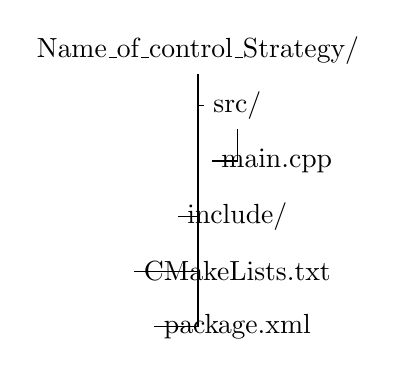
\begin{tikzpicture}[%
	grow via three points={one child at (0.5,-0.7) and
		two children at (0.5,-0.7) and (0.5,-1.4)},
	edge from parent path={(\tikzparentnode.south) |- (\tikzchildnode.west)}]
	\node {Name\_of\_control\_Strategy/}
	child { node {src/}
		child { node {main.cpp}}
	}
	child [missing] {}
	child { node {include/}}		
	child { node {CMakeLists.txt}}
	child { node {package.xml}};
	\end{tikzpicture}
	\caption{Organização do diretório de projeto de estratégias de controle. Os diretórios são dados pelas ''caixinhas'' com nomes terminados pelo caractere ''/'' e os arquivos possuem alguma extensão em seu nome.}
	\label{pacote}
\end{figure}


%\noindent
%Obs.: Os diretórios são dados pelas ''caixinhas'' com nomes terminados pelo caractere ''/'', e os arquivos possuem alguma extensão em seu nome.


\begin{itemize}
	\itemsep0em 
	\item[-]O arquivo ''main.cpp'' é o arquivo onde é implementada a lógica da estratégia de controle.
	\item[-]A pasta ''include'' armazena bibliotecas customizadas pelo usuário que são incluídas no preâmbulo do arquivo main.cpp.
	\item[-]O arquivo ''CMakeLists.txt'' fornece ao compilador informações sobre o diretório de bibliotecas incluídas nos códigos fontes do simulador. Detalhes sobre como incluir novas bibliotecas podem ser encontrados no Apêndice \ref{cmake}.
	\item[-]O arquivo ''package.xml'' é o arquivo necessário para armazenar dados como nome do autor, endereço de e-mail, etc. Detalhes de sua configuração são apresentados no Apêndice \ref{package}.
\end{itemize}



\section{Interface padrão para desenvolvimento de estratégias de controle e template main.cpp}

A criação de uma estratégia de controle é realizada através de herança da classe virtual padrão "IController". Sendo essa uma classe virtual, seus métodos precisam ser implementadas na classe filha. A Figura \ref{interface} ilustra suas funções métodos. 

A função método  \textit{config()} é executada no inicio das simulações, sendo utilizada para realizar configurações iniciais da estratégia de controle. O método \textit{execute()} é chamado pelo simulador a cada período de amostragem. Ele é \textbf{o método que deve conter toda a lógica da estratégia de controle}. A ordem e quantidade dos sinais entrada e saída desta função é determinada na interface como descrito na subseção \ref{sensoresatuadores}. As funções \textit{state()}, \textit{error()} e \textit{reference()} são métodos que retornam os valores dos sinais de erro, referência e sensores para serem armazenados em arquivos de texto. Os dados salvos nos arquivos txt podem ser utilizado para produzir gráficos dos resultados da simulação, utilizando o matlab, por exemplo. 



%A estratégia de controle deve ser implementada através de uma classe que herda uma interface padrão de comunicação com o ambiente de simulação, chamada IController, que está ilustrada na Figura \ref{interface}.

\begin{figure}[!ht]
\begin{minted}{cpp}
#ifndef ICONTROLLER_HPP
#define ICONTROLLER_HPP

#include "simulator_msgs/SensorArray.h"

class Icontroller 
{
	public:
	Icontroller(){};
	virtual ~Icontroller(){};
	virtual void config()=0;
	virtual std::vector<double> execute(simulator_msgs::SensorArray)=0;
	virtual std::vector<double> Reference()=0;
	virtual std::vector<double> Error()=0;
	virtual std::vector<double> State()=0;
};

extern "C" {
	typedef Icontroller* create_t();
	typedef void destroy_t(Icontroller*);
}
#endif
\end{minted}
\caption{Interface de implementação de estratégias de controle.}
\label{interface}
\end{figure}

%Esta interface orienta ao usuário os métodos virtuais necessários de se implementar. 

Quando uma nova estratégia de controle é criada, o ambiente de simulação fornece um arquivo main.cpp como template básico para a implementação da estratégia de controle. O conteúdo deste arquivo está ilustrado na Figura \ref{template}. A próxima seção apresenta um exemplo de implementação de estratégia de controle.

\begin{figure}[!ht]
\begin{minted}{cpp}
#include "Icontroller.hpp"

class demonstracao : public Icontroller
{
	public: demonstracao(){}
	public: ~demonstracao(){}
	public: void config(){}
	public: std::vector<double> execute(simulator_msgs::SensorArray arraymsg)
	{
		std::vector<double> out;
		return out;
	}
	public: std::vector<double> Reference()
	{
		std::vector<double> out;
		return out;
	}
	public: std::vector<double> Error()
	{
		std::vector<double> out;
		return out;
	}
	public: std::vector<double> State()
	{
		std::vector<double> out;
		return out;
	}
};

extern "C"
{
	Icontroller *create(void) {return new demonstracao;}
	void destroy(Icontroller *p) {delete p;}
}
\end{minted}
\caption{Template para implementação de estratégias de controle.}
\label{template}
\end{figure} 

\section{Exemplo de implementação de estratégia de controle}
\label{exemplo}

Esta seção demonstra o processo de implementação de uma nova estratégia de controle. Nela é apresentado um exemplo de utilização da interface gráfica para a criação e modificação de uma nova estratégia de controle, e também o processo de compilação. O exemplo utilizado corresponde à implementação de uma estratégia de controle robusto para rastreamento de trajetória da carga, transportada por um VANT na configuração Tilt-rotor. Mais detalhes da estratégia de controle pode ser encontrados em \cite{Lara2017}.


\subsection{Configurando a lista de sensores e atuadores disponíveis}

Na janela descrita na Seção \ref{SecEstCtrl}, ao selecionar a aba Sensors ou Actuator, uma das janelas illustrada na Figura \ref{abas} aparecerá. Em ambas, o usuário pode adicionar e remover instrumentos da lista utilizando os botões ''Add'' e ''Remove''. Além disso, clicando duas vezes sobre um nome na lista, é possível editar as propriedades do instrumento. Estas listas são de fundamental importância para a implementação da estratégia de controle, tais instrumentos e sua respectiva ordem definirão os dados de entrada e saída do controlador.

\begin{figure}[h!]
	\hfill
	\subfloat{\includegraphics[width=230pt]{figuras/6.png}}
	\hfill
	\subfloat{\includegraphics[width=230pt]{figuras/7.png}}
	\hfill
	\caption{Abas Sensors e Actuators.}
	\label{abas}
\end{figure}

Neste exemplo, o controlador receberá um vetor de sensores, no entanto contendo informações fornecidas por um único sensor, cujo tópico de comunicação é denominado ''Estados''. Além disso, o controlador deverá  retornar um vetor de ponto flutuante de dimensão 4 com sinais de entrada de controle para atuadores, cujos tópicos de comunicação estão na seguinte ordem: 1) Thrustdir, 2) Thrustesq, 3) RefaR e 4) RefaL.

\subsection{Criando uma nova estratégia de controle}

Para criar uma nova estratégia de controle, na aba Controller, pressione ''New Controller''. Uma nova janela será mostrada solicitando ao usuário o nome do novo controlador. Neste exemplo, a estratégia de controle terá o nome ''vant2load\_hinfinity'' (Figura \ref{projeto1}). Depois de confirmar o nome do controlador, uma janela do Nautilus aparecerá com o diretório do projeto criado (Figura \ref{2a}).

\begin{figure*}[!ht]
	\centering
	\includegraphics[width=0.7\columnwidth]{figuras/1a1a1.png}
	\caption{Criando uma nova estratégia de controle.}
	\label{projeto1}
\end{figure*}

\begin{figure*}[!ht]
	\centering
	\includegraphics[width=0.7\columnwidth]{figuras/2a.png}
	\caption{Arquivos e diretórios associados à nova estratégia de controle.}
	\label{2a}
\end{figure*}

\subsection{Implementação da estratégia de controle}

A Figura \ref{exemplo1} mostra um exemplo de código de estratégia de controle implementada no arquivo main.cpp. No exemplo, observa-se que é necessário a inclusão de 3 bibliotecas: 

\begin{figure}
\begin{minted}{cpp}
#include "Icontroller.hpp"
#include <Eigen/Eigen>
#include "simulator_msgs/Sensor.h"
	
class hinfinity : public Icontroller 
{
	private: Eigen::VectorXd Xref; // vetor de referência
	private: Eigen::VectorXd Erro; // vetor de erros
	private: Eigen::VectorXd Input; // sinais de controle
	private: Eigen::MatrixXd K; // matriz de ganhos do controlador
	private: Eigen::VectorXd X; // vetor de estados
	private: double T; // Período de amostragem
	
	public: hinfinity(): Xref(24), K(4,24), X(24), Erro(24), Input(4)
	{ 
		T = 0.012;
	}
	public: ~hinfinity(){	}
	
	public: void config()
	{	
		K<< [...] Dados da matriz [...];
	}
	public: std::vector<double> execute(simulator_msgs::SensorArray arraymsg)
	{
		static float count = 0;
		static float xint, x_ant = 0;
		static float yint, y_ant = 0;
		static float zint, z_ant = 0;
		static float yawint, yaw_ant = 0;
		// selecionando dados
		int i = 0;		
		simulator_msgs::Sensor msgstates;
		msgstates = arraymsg.values.at(0);		
		// Referência
		float trajectoryRadius = 2;
		float trajectoryHeight = 4*trajectoryRadius;
		float trajTime = 80;
		float pi = 3.14;
		float x = trajectoryRadius*cos((count*T)*2*pi/trajTime);
		float xdot = -trajectoryRadius*(2*pi/trajTime)*sin((count*T)*2*pi/trajTime);
		float xddot = -trajectoryRadius*(2*pi/trajTime)*(2*pi/trajTime)
				*cos((count*T)*2*pi/trajTime);
		float y = trajectoryRadius*sin((count*T)*2*pi/trajTime);
		float ydot = trajectoryRadius*(2*pi/trajTime)*cos((count*T)*2*pi/trajTime);
		float yddot = -trajectoryRadius*(2*pi/trajTime)*(2*pi/trajTime)
				*sin((count*T)*2*pi/trajTime);
		float z = trajectoryHeight+1 - trajectoryHeight*cos((count*T)*2*pi/trajTime);
		float zdot = trajectoryHeight*(2*pi/trajTime)*sin((count*T)*2*pi/trajTime);
		float zddot = trajectoryHeight*(2*pi/trajTime)*(2*pi/trajTime)
				*cos((count*T)*2*pi/trajTime);
		Xref << x,y,z,0,0,0,0.00002965,0.004885,0.004893,0.00484,xdot,ydot,zdot,
			0,0,0,0,0,0,0,0,0,0,0;
		
		\end{minted}
		\end{figure}
		\begin{figure}
		\begin{minted}{cpp}
		//Convertendo velocidade angular
		std::vector<double> etadot = pqr2EtaDot(msgstates.values.at(13),
		msgstates.values.at(14),
		msgstates.values.at(15),
		msgstates.values.at(3),
		msgstates.values.at(4),
		msgstates.values.at(5));
		
		// Integrador Trapezoidal
		float x_atual = msgstates.values.at(0) - Xref(0);
		xint = xint + (T/2)*(x_atual + x_ant);
		x_ant = x_atual;
		float y_atual = msgstates.values.at(1) - Xref(1);
		yint = yint + (T/2)*(y_atual + y_ant);
		y_ant = y_atual;
		float z_atual = msgstates.values.at(2) - Xref(2);
		zint = zint + (T/2)*(z_atual + z_ant);
		z_ant = z_atual;
		float yaw_atual = msgstates.values.at(5) - Xref(5);
		yawint = yawint + (T/2)*(yaw_atual + yaw_ant);
		yaw_ant = yaw_atual;
		
		// vetor de estados aumentado
		X << msgstates.values.at(0),//x
		msgstates.values.at(1),//y
		msgstates.values.at(2),//z
		msgstates.values.at(3),//roll
		msgstates.values.at(4),//pitch
		msgstates.values.at(5),//yaw
		msgstates.values.at(8),//g1 x
		msgstates.values.at(9),//g2 y
		msgstates.values.at(6),//aR
		msgstates.values.at(7),//aL
		msgstates.values.at(10),//vx
		msgstates.values.at(11),//vy
		msgstates.values.at(12),//vz
		etadot.at(0),//droll
		etadot.at(1),//dpitch
		etadot.at(2),//dyaw
		msgstates.values.at(18), // angulo da primeira junta da carga
		msgstates.values.at(19), // angulo da segunda junta da carga
		msgstates.values.at(16), // derivada do angulo da primeira junta da carga
		msgstates.values.at(17), // derivada do angulo da segunda junta da carga
		xint,
		yint,
		zint,
		yawint;
		
		
		// lei de controle
		Erro = X-Xref;
		Input = -K*Erro;
		
		\end{minted}
		\end{figure}
		\begin{figure}
		\begin{minted}{cpp}
		
		// Criando vetor com dados da trajetória de referência
		Eigen::MatrixXd qref(10,1);
		qref << x,y,z,0,0,0,0.00002965,0.004885,0.004893,0.00484;
		Eigen::MatrixXd qrefdot(10,1);
		qrefdot << xdot,ydot,zdot,0,0,0,0,0,0,0;
		Eigen::MatrixXd qrefddot(10,1);
		qrefddot << xddot,yddot,zddot,0,0,0,0,0,0,0;
		
		// Feedforward
		Input(0) = Input(0) + 12.6005;
		Input(1) = Input(1) + 12.609;
		count++; 
		
		
		// convertendo dados do vetor da biblioteca Eigen para vetor a biblioteca padrão de C++
		std::vector<float> out2(Input.data(), Input.data() + Input.rows() 
					* Input.cols());
		
		std::vector<double> out(out2.size());
		for(int i=0; i<out2.size();i++) out.at(i) = out2.at(i);
		return out;
	}
	
	public: std::vector<double> Reference()
	{
		std::vector<double> out(Xref.data(), Xref.data() + Xref.rows() 
					* Xref.cols());
		return out;
	}
	
	public: std::vector<double> Error()
	{
		std::vector<double> out(Erro.data(), Erro.data() + Erro.rows() 
					* Erro.cols());	
		return out;
	}	
	
	public: std::vector<double> State()
	{
		std::vector<double> out(X.data(), X.data() + X.rows() * X.cols());
		return out;
	}
	
	private: std::vector<double> pqr2EtaDot(double in_a, double in_b, double in_c, 
						double phi, double theta, double psii)
	{
		std::vector<double> out;
		out.push_back(in_a + in_c*cos(phi)*tan(theta) + in_b*sin(phi)*tan(theta));
		out.push_back(in_b*cos(phi) - in_c*sin(phi));
		out.push_back((in_c*cos(phi))/cos(theta) + (in_b*sin(phi))/cos(theta));
		return out;
	}
};
	
	\end{minted}
	\end{figure}
	\begin{figure}
	\begin{minted}{cpp}
	
extern "C"
{ 
	Icontroller *create(void) {
		return new hinfinity;
	}
	void destroy(Icontroller *p) {
		delete p;
	}
}
\end{minted}
\caption{Exemplo de código.}
\label{exemplo1}
\end{figure}

\begin{itemize}
		\setlength{\itemsep}{1pt}
		\setlength{\parskip}{0pt}
		\setlength{\parsep}{0pt}
\item \#include ''Icontroller.hpp''  - informa ao código a interface padrão para criação de controladores no ambiente de simulação;
\item \#include <Eigen/Eigen> - importa as funcionalidades fornecidas pela biblioteca Eigen \footnote{https://eigen.tuxfamily.org}. A biblioteca Eigen fornecer funções para realizar operações da álgebra linear;
\item \#include ''simulator\_msgs/Sensor.h'' - informa a classe responsável por abstrair o padrão de comunicação entre o controlador e os sensores.
\end{itemize}


Os atributos \textbf{Xref}, \textbf{Erro}, \textbf{Input}, \textbf{K} e \textbf{X} são as estruturas de de vetores e matrizes da biblioteca Eigen. Essas estruturas são responsáveis por realizar a operações de álgebra linear e, portanto, permitir a relização da lei de controle. O atributo \textbf{T} determina o período de amostragem do controlador.

O construtor hinfinity() inicializa os atributos da classe, enquanto o destrutor \textasciitilde hinfinity() não possui nenhuma função no contexto do simulador.

Neste exemplo, o método config() é utilizado para atribuir valores à matriz de ganhos K, respeitando a sintaxe da biblioteca Eigen, no entanto o usuário pode utilizar esse espaço para realizar qualquer outra configuração inicial. Por fim, a lógica da estratégia de controle é implementada no método execute(), que é executado a cada período de amostragem, como descrito anteriormente.

O código começa por declarar as variáveis (estáticas) ''xint'', ''x\_ant'', ''yint'', ''y\_ant'', ''zint'', ''z\_ant'', ''yawint'' e ''yaw\_ant'', utilizadas para armazenar os valores dos integradores implementados na estratégia de controle. Em seguida, está presente o trecho de código referente aos dados dos sensores, obtidos através do vetor ''arraymsg''. Como neste exemplo somente um sensor está disponível (''Estados''), apenas a primeira posição deste vetor é acessada (através da sintaxe ''arraymsg.values.at(0)''). Nos casos em que mais sensores são disponibilizados, os dados do n-ésimo sensor são acessados através de  ''arraymsg.values.at(n-1)'' e a ordem desse vetor é definida a priori na aba Sensor conforme é visualizada em \ref{6}. Em seguida, é definido a referência para o controlador e implementado integradores, através do método de integração trapezoidal, para realização da lei de controle e, por fim, é calculada a ação de controle feedforward. 

Os métodos Reference(), Error(), State() são utilizados para armazenar dos sinais de referência, erro e estados, respectivamente, nos arquivos de texto de saída do ambiente de simulação. A função pqr2EtaDot() corresponde a um mapeamento de parte das informações recebidas pelos sensores, necessário para a implementação da estratégia de controle deste exemplo. 

Assim como a função pqr2EtaDot(), quaisquer funções adicionais que sejam necessárias para a implementação da estratégia de controle, podendo estar relacionadas também a algoritmos de filtragem, podem ser escritas dentro da classe ''main.cpp'', ou em classes auxiliares criadas dentro da pasta ''include'' ilustrada em \ref{2a} (neste caso, estas devem ser também incluídas no cabeçalho do arquivo ''main.cpp'').


Por fim, o trecho de código a seguir corresponde à funções necessárias para garantir o carregamento da estratégia de controle em tempo de execução do simulador. O método create() cria uma instância da classe que encapsula o controlador, e o método destroy() é utilizado para destruir a instância da classe.

\begin{minted}{cpp}
extern "C"
{ 
	Icontroller *create(void) {
		return new hinfinity;
	}
	void destroy(Icontroller *p) {
		delete p;
	}
}
\end{minted}


%\subsection{Configurando CMakeLists.txt}
%
%Em seguida, substitua o código template do CMakeLists.txt com o seguinte código.
%
%
%\begin{minted}{xml}
%cmake_minimum_required(VERSION 2.8.3)
%project(vant2load_hinfinity)
%
%find_package(catkin REQUIRED COMPONENTS
%			roscpp
%			simulator_msgs)
%	
%include_directories(include)
%INCLUDE_DIRECTORIES (/usr/include/eigen3)
%include_directories( ${catkin_INCLUDE_DIRS})
%include_directories($ENV{TILT_PROJECT}/source/Structure/control_strategies/)
%
%add_library(vant2load_hinfinity src/hinfinity.cpp)
%target_link_libraries(vant2load_hinfinity ${catkin_LIBRARIES})
%install(TARGETS
%vant2load_hinfinity
%ARCHIVE DESTINATION ${CATKIN_PACKAGE_LIB_DESTINATION}
%LIBRARY DESTINATION ${CATKIN_PACKAGE_LIB_DESTINATION}
%RUNTIME DESTINATION ${CATKIN_PACKAGE_BIN_DESTINATION})
%\end{minted}
%
%
%\subsection{Configurando package.xml}
%
%Em seguida, substitua o código template do package.xml com o seguinte código.
%
%\begin{minted}{xml}
%<?xml version="1.0"?>
%<package>
%	<name>vant2load_hinfinity</name>
%	<version>1.0.0</version>
%	<description>The hinfinity package</description>
%	
%	<maintainer email="macro@todo.todo">macro</maintainer>
%	<license>TODO</license>
%	
%	<buildtool_depend>catkin</buildtool_depend>
%	<build_depend>roscpp</build_depend>
%	<run_depend>roscpp</run_depend>
%	<build_depend>simulator_msgs</build_depend>
%	<run_depend>simulator_msgs</run_depend>
%	
%	<export>
%	</export>
%
%</package>
%\end{minted}
%
%O arquivo package.xml deste exemplo informa que o nome do pacote que encapsula o projeto de controle é denominada de "vant2load_hinfinity"

\subsection{Compilando o código da estratégia de controle}

Após a implementação da estratégia de controle, o código correspondente pode ser compilado através do botão ''Compile'' (conforme explicado no Capítulo 2, vide Figura \ref{5}, item 4).

%\chapter{Inserção de novo cenário}
%
%Um cenário no Gazebo é uma instância de simulação composto por um ou mais modelos incluídos. Este ambiente de simulação está formatado para o funcionamento de apenas um VANT, sendo que demais modelos incluídos são ilustrativos. Há duas maneiras de se incluir um novo cenário: cenário template e cenário editável e pronto para simular. 
%
%O cenário template é a criação de um arquivo com sufixo ".tpl" que tenha apenas elementos ilustrativos e não seja editável pela interface gráfica de configuração. Já o outro é um cenário pronto para uso com VANT definido com sufixo ".world". A estrutura organizacional de ambos os cenários está ilustrado a seguir:
%
%
%\begin{lstlisting}
%<?xml version="1.0" encoding="UTF-8"?>
%<sdf version="1.6">
%	<world name="/home/macro/catkin_ws/src/provant_simulator/source/Database/simulation_elements/worlds/templates/empty/empty2.tpl">
%		<gravity>0.000000 0.000000 -9.8000</gravity>
%		<physics type="ode">
%			<max_step_size>0.001000</max_step_size>
%			<real_time_factor>0</real_time_factor>
%		</physics>
%		<plugin name="gazebo_tutorials" filename="libgazebo_ros_world_plugin.so"/>
%		<include>
%			<uri>model://ground_plane</uri>
%			<static>false</static>
%		</include>
%		<include>
%			<uri>model://sun</uri>
%			<static>false</static>
%		</include>
%		<include>
%			<uri>model://vant_2.0</uri>
%			<name>newmodel</name>
%			<static>false</static>
%			<pose>0 0 2 0 0 0</pose>
%		</include>
%		<scene>
%			<sky>
%				<time>18</time>
%				<clouds>
%					<speed>0</speed>
%				</clouds>
%			</sky>
%		</scene>
%	</world>
%</sdf>
%\end{lstlisting}
%
%onde,
%
%\begin{itemize}
%	\setlength{\itemsep}{1pt}
%	\setlength{\parskip}{0pt}
%	\setlength{\parsep}{0pt}
%	\item[-] <gravity></gravity> valores de definição do vetor de aceleração da gravidade (em $metros/s^2$).
%	\item[-] atributo "type" da tag physics : especifica qual motor de simulação será utilizado 
%	\item[-] <physics><max\_step\_size></max\_step\_size></physics> valor do passo de simulação (em milissegundos)
%	\item[-] <physics><real\_time\_factor><real\_time\_factor></max\_step\_size><physics> valor 1 define que o Gazebo tentará funcionará em tempo real e 0 define que o Gazebo funcionará o mais rápido possível. 
%	\item[-] <plugin></plugin> definição do plugin mundo com a função de sincronização da simulação;
%	\item[-] <include><uri></uri></include> nome do modelo a ser incluído no cenário
%	\item[-] <include><static></static></include> define se o modelo terá dinâmica simulada pelo motor de simulação
%	\item[-] <include><name></name></include> nome do modelo
%	\item[-] <include><pose></pose></include> pose inicial do modelo na simulação
%	\item[-] <scene><time></time></scene> hora do dia q a simulação simulará
%	\item[-] <scene><clouds><speed></speed></clouds></scene> inclusão de nuvens na simulação e sua respectiva velocidade
%\end{itemize}
%
%Obs.: Esta versão do ambiente de simulação está preparado para receber apenas essas configurações. Não adicione outros tipos de informação. 
%  
%


%

%
%\chapter{Arquitetura de software}
%
%\section{Malha de controle}
%
%A malha de controle desenvolvida neste trabalho está ilustrada na Figura x e é composta por um nó Controlador. O nó Controlador é o local obtém as informações sensoriais, coloca na ordem pre-definida pelo usuário, executa a lei de controle e envia os sinais de controle para o simulador. Assim que o modelo recebe os novos comandos, é realizado um novo passo de simulação, fechando o laço de comunicação.
%
%\begin{figure}[!htb]
%	%\vspace{-3mm}
%	\centering{
%		\def\svgwidth{0.745\columnwidth}
%		%{\footnotesize\import{Figuras/}{simulator_flowchart.pdf_tex}}%\vspace{-1mm}
%		{\footnotesize\import{figuras/}{simulator_flowchartV2.pdf_tex}}%\vspace{-1mm}
%		%\caption{Fluxo de funcionamento do ambiente de simulação.}\label{flow}}%kinematics}}
%		%\caption{Estrutura do ambiente de simulação.}\label{flow}}%kinematics}}
%		\caption{Fluxo de informações do ambiente de simulação.}\label{flow}}%kinematics}}
%	%\vspace{-3mm}
%\end{figure}
%
%\section{Interface Gráfica}
%
%O código desenvolvido está organizado em três níveis de modularização: “camada de acesso a dados”, “camada de negócios” e ”camada de apresentação”. A Figura x ilustra esta organização. Esses níveis proveem facilidade de manutenção do código e desacoplamento de funcionalidades.
%
%Na “camada de acesso a dados” estão as classes responsáveis por ler e escrever em arquivos XML. Nesse nível de desenvolvimento utilizou-se o módulo de software QXml fornecida pela API do ambiente de desenvolvimento QT para ter acesso à hierarquia de informações do arquivo XML. Na “camada de negócios”, encontram-se as classes responsáveis por descrever a estrutura de dados onde são armazenados os detalhes de configuração dos modelos. Já a “camada de apresentação” define a apresentação e as funcionalidades da interface gráfica.
%
%\begin{figure*}[!ht]
%	\centering
%	\includegraphics[width=100pt]{figuras/threelayers.jpeg}
%	\caption{Arquitetura de software da interface gráfica}
%	\label{7}
%\end{figure*}
%
%%\appendix
%
%%\chapter{ROS}
\appendix

\chapter{Models}
\label{newmodel}

The files associated with the UAV models used in ProVANT Simulator are located in the following path:

\begin{bashcode}
	$HOME/catkin_ws/src/provant_simulator/source/Database/simulation_elements/models/real
\end{bashcode}

Each model in the simulation environment has a directory with its respective name. This directory contains files that describe the dyanmic, visual, collision and sensorial models, and the control law used. Thus, in case it's necessary to add a new model, or edit an existing one, it must have the UAV's configuration/description files organized as depicted in Figure \ref{modeloorg}.\\

\begin{figure}[H]
	\centering \tt
	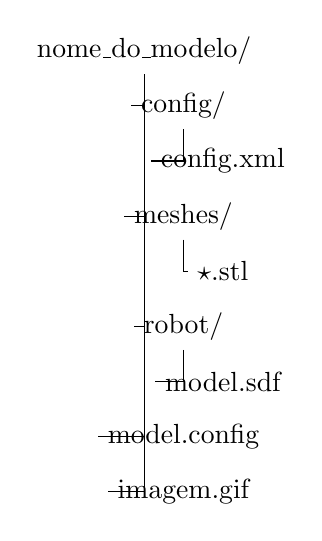
\begin{tikzpicture}[%
		grow via three points={one child at (0.5,-0.7) and
			two children at (0.5,-0.7) and (0.5,-1.4)},
		edge from parent path={(\tikzparentnode.south) |- (\tikzchildnode.west)}]
		\node {nome\_do\_modelo/}
		child { node {config/}
			child { node {config.xml}}
		}
		child [missing] {}
		child { node {meshes/}
			child {node {$\star$.stl}}
		}
		child [missing] {}
		child { node {robot/}
			child { node {model.sdf}}
		}
		child [missing] {}
		child { node {model.config}}
		child { node {imagem.gif}};
	\end{tikzpicture}
	\caption{Directory's organization with UAV model description files}
	\label{modeloorg}
\end{figure}

where:

\begin{enumerate}
	\item File \verb config.xml  stores the information regarding the controller to be used in the model.
	\item File \verb model.config  describes thte UAV's dynamic, collision and visual models for simulator Gazebo.
	\item File \verb model.config  describes the model's metadata.
	\item File \verb imagem.gif  contains the image used by the garphical interface to illustrate the UAV model (see Figure \ref{tela_inicial.jpg}, item 2).
	\item The directory \verb meshes  stores the files exported from the CAD tool (used for the UAV's mechanical design), like SolidWorks.
\end{enumerate}

The file \verb model.config  tells Gazebo where is the file with the model's strucutal data and provides information regarding the models's author, version and description. Figure \ref{model.config} illustrates an example of this file. The tags used in \verb model.config  are:

\small
\begin{itemize}
	\setlength{\itemsep}{1pt}
	\setlength{\parskip}{0pt}
	\setlength{\parsep}{0pt}
	\xmlfield{name}{The model's name}
	\xmlfield{version}{The model's version}
	\xmlfield{sdf}{Path to the file that describes the Gazebo model's dynamic, colision and visual characteristics}
	\item[-] \textcolor{blue}{\texttt{<author>}}
	\begin{itemize}
		\xmlfield{name}{The author's name}
		\xmlfield{email}{Author's email adress}
	\end{itemize}
	\textcolor{blue}{\texttt{</author>}}
	\xmlfield{description}{Brief description of the model}
\end{itemize}
\normalsize

\begin{code}[H]
	\begin{minted}[obeytabs=true,tabsize=4]{xml}
		<?xml version="1.0"?>
		<model>
			<name>vant</name>
			<version>1.0</version>
			<sdf version='1.5'>robot/model.sdf</sdf>
			<author>
				<name>provant</name>
				<email>provant@ufmg.br</email>
			</author>
			<description>
				The UAV version 3.0 of the provant project 
			</description>
		</model>
	\end{minted}
	\caption{Example content for file \texttt{model.config}}
	\label{model.config}
\end{code}

The file \verb config.xml  stores all the settings regarding the control structure to be used during the simulation, such as sensors, actuatores, control laws and sampling period. ith the purpose of helping the user to edit this file, the graphical interface provides tools for this task, so that the user won't have to directly access this file. Code \ref{config.xml} illustrates an example of this file:

\begin{code}[H]
	\begin{minted}[obeytabs=true,tabsize=4]{xml}
		<?xml version="1.0" encoding="UTF-8"?>
		<config>
			<TopicoStep>Step</TopicoStep>
			<Sampletime>12</Sampletime>
			<Strategy>libvant3_lqr.so</Strategy>
			<RefPath>ref.txt</RefPath>
			<Outputfile>out.txt</Outputfile>
			<InputPath>in.txt</InputPath>
			<ErroPath>erro.txt</ErroPath>
			<Sensors>
				<Device>Estados</Device>
			</Sensors>
			<Actuators>
				<Device>ThrustR</Device>
				<Device>ThrustL</Device>
				<Device>TauR</Device>
				<Device>TauL</Device>
				<Device>Elevdef</Device>
				<Device>Ruddef</Device>
			</Actuators>
		</config>
	\end{minted}
	\caption{Example of \texttt{config.xml} file}
	\label{config.xml}
\end{code}

The tags used in file \verb config.xml  are:

\small
\begin{itemize}
	\setlength{\itemsep}{1pt}
	\setlength{\parskip}{0pt}
	\setlength{\parsep}{0pt}
	\xmlfield{TopicoStep}{The sincronization topic between the simulator and the controller. \textbf{This tag's value must not be changed.}}
	\xmlfield{Sampletime}{The controller's smapling period, in milliseconds}
	\xmlfield{Strategy}{Name of the library associated to the implementation of the control strategy to be used along with this model}
	\xmlfield{RefPath}{Name of the file where the setpoint signal data is stored}
	\xmlfield{Outputfile}{Name of the file where the control signal data is stored}
	\xmlfield{InputPath}{Name of the file where the sensor data is stored}
	\xmlfield{ErroPath}{Name of the file where the error vector data is stored}
	\xmlfield{Sensors}{Name of the sensor topics to which the control strategy will have access (in the specified order)}
	\xmlfield{Actuators}{Name of the actuator topics to which the control strategy will have access (the controller must return a vector with the same amount of data and in the order specified here)}
\end{itemize}
\normalsize

File \verb model.sdf  provides to Gazebo the UAV model's information in XML format following the \href{http://sdformat.org/spec}{SDF format} (Figure \ref{geral} illustrates an example of this file). The next section describes more thoroughly the basic structure of an SDF file.

\section{The SDF file}

Before presenting the basic configuration of an SDF file, it's necessary to introduce a few concepts.

In the simulator, a model correspond to a mechanical system, which can be formed my one or multiple rigid bodies\footnote{By assuming a body as rigid, the elasticity and deformation effects are neglected}. Thus, as in a manipulator, the bodies in the simulator are called links. Child links are connected to parent links by joints. Child links are rigid bodies whose movements are restricted by the connection (joint) with bodies called parent links. The links have inertial, visual and collision properties.

As for joints, they impose restrictions to the relative movement between two links and have properties such ase joint type (prismatic, revolute, etc.), movement limits (position ans speed), friction, etc. Code \ref{geral} illustrates an example of an SDF file.

\begin{code}[H]
	\begin{minted}[obeytabs=true,tabsize=4]{xml}
		<?xml version="1.0" encoding="UTF-8"?>
		<sdf version="1.4">
			<model name="modelo">
				<link name="corpo">
					...
				</link>
				<link name="servo">
					...
				</link>
				<joint name="corpo_servo">
					...
				</joint>
			</model>
		</sdf>
	\end{minted}
	\caption{Description of a model in file \texttt{model.sdf}}
	\label{geral}
\end{code}

The tags used are:

\small
\begin{itemize}
	\setlength{\itemsep}{1pt}
	\setlength{\parskip}{0pt}
	\setlength{\parsep}{0pt}
	\xmlfield{link}{Describes a link, specifying its name}
	\xmlfield{joint}{Describes a joint, specifying its name}
\end{itemize}\normalsize

Each link in the model has trhee types of description for the simulator: the kinematic, visual and collision descriptions. The configuration structure of a link in an SDF file has athe format depicted in code \ref{elo}:

\begin{code}[H]
	\begin{minted}[obeytabs=true,tabsize=4]{xml}
		<link name="servodir">
			<pose>0.02E-3 -277.61E-3 56.21E-3 -0.0872665 0 0</pose>
			<inertial> 
				...
			</inertial>
			<collision name="servodircollision"> <!--opcional-->
				...
			</collision>
			<visual name="servodirvisual"> <!--opcional-->
				...
			</visual>
		</link>
	\end{minted}
	\caption{Description of a link in file \texttt{model.sdf}}
	\label{elo}
\end{code}

The tags used are:

\small
\begin{itemize}
	\setlength{\itemsep}{1pt}
	\setlength{\parskip}{0pt}
	\setlength{\parsep}{0pt}
	\xmlfield{pose}{Link's pose}
	\xmlfield{inertial}{Link's inertial properties}
	\xmlfield{collision}{Link's collision properties. The collision models for the UAVs used in the simulation environment are obtained from CAD files.}
	\xmlfield{visual}{Visual characteristics such as color and shape. The visual models for the UAVs used in the simulation environment are obtained from CAD files, except for the color, which is specified separately.}
\end{itemize}
\normalsize

\noindent \textbf{Links inertial parameters:} The user must inform each link's inertial parameters inside the tag \verb inertial . The required information are the mass, the center of mass' relative position and the inertia tensor. In Code \ref{inertial} an exemple configuration of a link's inertial parameters in format SDF is illustrated.

\begin{code}[H]
	\begin{minted}[obeytabs=true,tabsize=4]{xml}
		<inertial>
			<mass>0.0809439719362664</mass>
			<pose>
				-3.60859273452335E-10 -0.000226380714807978 0.0594780519701684 0 0 0
			</pose>
			<inertia>
				<ixx>3.88267747087835E-06</ixx>
				<ixy>6.03219085082653E-06</ixy>
				<ixz>-2.78471406661236E-12</ixz>
				<iyy>0.000104858690365283</iyy>
				<iyz>7.0486590219062E-07</iyz>
				<izz>8.31755564684115E-05</izz>		
			</inertia>
		</inertial>
	\end{minted}
	\caption{Description of inertial characteristics in file \texttt{model.sdf}}
	\label{inertial}
\end{code}

The tags used are:

\small
\begin{itemize}
	\setlength{\itemsep}{1pt}
	\setlength{\parskip}{0pt}
	\setlength{\parsep}{0pt}
	\xmlfield{mass}{The link's mass}
	\xmlfield{pose}{The center of mass' position relative to its main coordinate system}
	\xmlfield{inertia}{The link's inertia tensor}
\end{itemize} 
\normalsize

\noindent \textbf{Link's collision properties:} In order for collision effects to be applied to the link, the user must describe the link's shape in file \verb model.sdf . There are many ways to describe it, but this guide presents only the method used in the UAV models in ProVANT Simulator, which consists of importing files created with CAD tools, such as SolidWorks. Code \ref{colision} shows an example descriptioin of a link's visual parameters using an STL file:

\begin{code}[H]
	\begin{minted}[obeytabs=true,tabsize=4]{xml}
		<collision name="servodircollision">
			<pose>0 0 0 0 0 0</pose>
			<geometry>
				<mesh>
					<uri>model://vant_2comcarga/meshes/servodir.STL</uri>
				</mesh>
			</geometry>
		</collision>
	\end{minted}
	\caption{Description of collision characteristics in file \texttt{model.sdf}}
	\label{colision}
\end{code}

The tags used are:

\small
\begin{itemize}
	\setlength{\itemsep}{1pt}
	\setlength{\parskip}{0pt}
	\setlength{\parsep}{0pt}
	\xmlfield{pose}{The collision model's pose relative to the link's coordinates' origin}
	\item[-] \textcolor{blue}{\texttt{<geometry>}}
	\begin{itemize}
		\item[-] \textcolor{blue}{\texttt{<mesh>}}
		\begin{itemize}
			\xmlfield{uri}{Path to the mesh file, relative to the model's directory, obtained by exporting from SolidWorks}
		\end{itemize}
		\textcolor{blue}{\texttt{</mesh>}}
	\end{itemize}
	\textcolor{blue}{\texttt{</geometry>}}
\end{itemize}
\normalsize

\noindent \textbf{Links visual properties:} In order for the link o be visualized during the simulation, the user must describe the link's visual parameters in file \verb model.sdf . Just like in the previous case, there are several description methods, but this guide illustrates only the one used in the simulation environment's UAVs, which consists of importing files created from CAD tools. Code \ref{visual} Shows an example description of a link's visual parameters using an STL file:

\begin{code}[H]
	\begin{minted}[obeytabs=true,tabsize=4]{xml}
		<visual name="servodirvisual">
			<pose>0 0 0 0 0 0</pose>
			<geometry>
				<mesh>
					<uri>model://vant_2comcarga/meshes/servodir.STL</uri>
				</mesh>
			</geometry>
			<material>
				<ambient>0 0 0 0</ambient>
				<diffuse>1 1 1 1</diffuse>
				<specular>0.1 0.1 0.1 1</specular>
				<emissive>0 0 0 0</emissive>
			</material>
		</visual>
	\end{minted}
	\caption{Description of visual characteristics in file \texttt{model.sdf}}
	\label{visual}
\end{code}

The tags used are:

\small
\begin{itemize}
	\setlength{\itemsep}{1pt}
	\setlength{\parskip}{0pt}
	\setlength{\parsep}{0pt}
	\xmlfield{pose}{The visual model's pose relative to the link's coordinates' origin}
	\item[-] \textcolor{blue}{\texttt{<geometry>}}
	\begin{itemize}
		\item[-] \textcolor{blue}{\texttt{<mesh>}}
		\begin{itemize}
			\xmlfield{uri}{Path to the mesh file, relative to the model's directory, obtained by exporting from SolidWorks}
		\end{itemize}
		\textcolor{blue}{\texttt{</mesh>}}
	\end{itemize}
	\textcolor{blue}{\texttt{</geometry>}}
	\item[-] \textcolor{blue}{\texttt{<material>}}
	\begin{itemize}
		\xmlfield{ambient}{Ambient color}
		\xmlfield{diffuse}{Diffuse color}
		\xmlfield{specular}{Specular color}
		\xmlfield{emissive}{Emissive color}
	\end{itemize}
	\textcolor{blue}{\texttt{</material>}}
\end{itemize} 
\normalsize

\subsection{Joint description} 

Ther joint types in the simulator are:

\begin{itemize}
	\item \textbf{revolute}: Rotation movement;
	\item \textbf{gearbox}: Revolute joint with transmission gears between links with different torque and speed ratios;
	\item \textbf{revolute2}: Joint composed by two revolute joints in series;
	\item \textbf{prismatic}: Prismatic joint;
	\item \textbf{universal}: Joint behaving as an articulated sphere;
	\item \textbf{piston}: Joint behaving as a combination of a revolute and a prismatic joint.
\end{itemize}

An example of a joint's configuration structure is shown in Code \ref{joint}.
\begin{code}[H]
	\begin{minted}[obeytabs=true,tabsize=4]{xml}
		<joint name="aR" type="revolute">
			<pose>0 0 0 0 0 0</pose>
			<parent>corpo</parent>
			<child>servodir</child>
			<axis>
				<xyz>0 0.9962 -0.0872</xyz>
				<limit>
					<lower>-1.5</lower>
					<upper>1.5</upper>
					<effort>2</effort>
					<velocity>0.5</velocity>
				</limit>
				<dynamics>
					<damping>0</damping>
					<friction>0</friction>
				</dynamics>
			</axis>
		</joint>
	\end{minted}
	\caption{Joint description in file \texttt{model.sdf}}
	\label{joint}
\end{code}
The tags used are:

\begin{itemize}
	\setlength{\itemsep}{1pt}
	\setlength{\parskip}{0pt}
	\setlength{\parsep}{0pt}
	\xmlfield{pose}{Child link's pose relative to the parent link}
	\xmlfield{parent}{Parent link's name}
	\xmlfield{axis}{Unit vector corresponding to the joint's rotation axis (expressed in the model's coordinate system if the SDF version is 1.4, or in the child link's coordinate system if the version is 1.6)}
	\xmlfield{lower}{Lower limit to the joint's position (in radians if it's a revolute joint or meters if it's prismatic)}
	\xmlfield{upper}{Upper limit to the joint's position (in radians if it's a revolute joint or meters if it's prismatic)}
	\xmlfield{velocity}{Joint's speed limit (in rad/s if it's a revolute joint or m/s if it's prismatic)}
	\xmlfield{effort}{Joint's effort limit (in N$\cdot$m if it's a revolute joint or N if it's prismatic)}
	\xmlfield{damping}{Vicous friction coefficient}
	\xmlfield{friction}{Static friction coefficient}
\end{itemize}

\subsection{Plugin description}
\label{plugins}

Plugins are dynamic libraries loaded during the simulator's initialization, using the configurations stored in the model description file (SDF file). These libraries are used to implement the sensors and actuators in the simulation environment.

ProVANT Simulator only uses two of \href{http://gazebosim.org/tutorials/?tut=plugins_hello_world}{Gazebo's plugin types} for the UAV model's control and monitoring: Model and Sensor.

\noindent \textbf{Model plugins:} Model plugins are dynamic libraries which control and monitor the UAV model's simulation variables. With them it's possible to create customized sensors and actuators. To insert a model plugin in file \verb model.sdf , the user must add \textcolor{blue}{\texttt{<plugin>}} tags defining its name, the dynamic library's name and the internal tags required to configure the plugin. Code \ref{pluginmod} exemplifies the insertion process.

The options for model plugins available in ProVANT Simulator are detailed in appendix \ref{pluginsAp}.

\begin{code}[H]
	\begin{minted}[obeytabs=true,tabsize=4]{xml}
		<?xml version="1.0" encoding="UTF-8"?>
		<sdf version="1.4">
			<model name="modelo">
				<link name="corpo">
					...
				</link>
				<link name="servo">
					...
				</link>
				<joint name="corpo_servo">
					...
				</joint>
				<plugin name="plugin_servo">
					...
				</plugin>
			</model>
		</sdf>
	\end{minted}
	\caption{Insertion of model plugins in file \texttt{model.sdf}}
	\label{pluginmod}
\end{code}

\noindent \textbf{Sensor plugins:} Sensor plugins are dynamic lybraries to simulate sensors, used by ProVANT Simulator to measure data from a UAV model. To insert sensor plugins, the user must add \textcolor{blue}{\texttt{<sensor>}} tags defining its name and the internal tags required to configure the plugin. Code \ref{pluginsen} exemplifies the insertion process.

\begin{code}[t]	
	\begin{minted}[obeytabs=true,tabsize=4]{xml}
		<link name="servodir">
			<pose>0.02E-3 -277.61E-3 56.21E-3 -0.0872665 0 0</pose>
			<inertial> 
				...
			</inertial>
			<collision name="servodircollision"><!--opcional-->
				...
			</collision>
			<visual name="servodirvisual"> <!--opcional-->
				...
			</visual>
			<sensor name="servosensor"> <!--opcional-->
				...
			</sensor>
			<sensor name="servosensor2"> <!--opcional-->
				...
			</sensor>
		</link>
	\end{minted}
	\caption{Insertion of sensor plugins in file \texttt{model.sdf}}
	\label{pluginsen}	
\end{code}

The sensor available in ProVANT Simulator are GPS, IMU, sonar and magnetometer (\href{http://sdformat.org/spec}{more details} on their configuration in file \verb model.sdf ). However, those sensors don't have a communication interface with ROS, since they broadcast their date via Gazebo topics. To broadcast these data to ROS topics the user must add, along with the sensor plugins, model plugins. Such plugins are specified in appendix \ref{pluginsAp}.

Note: In order for the sensor to work properly, the user must adjust the sampling rate to exactly the inverse of the simulation step (e.g. 1000~Hz).

\subsection{Communication messages' standard}

As a standard, all plugins and sensor available in the simulation environment make their provide their data using the same data structure. This data structure is abstracted in ROS through messages. Messages are simple data structures containing typed fields. The sensor plugins' standard message is illustrated below, where:

\begin{itemize}
	\item \verb header : provides the time instant in which the data as obtained, the frame and the sequential ID
	\item \verb name : provides the name of the instrument which provided the message
	\item \verb values : vector containing the data provided by the sensors
\end{itemize} 

\begin{code}[H]
	\begin{verbatim}
		- Header header
		- string name
		- float64[] values
	\end{verbatim}	
\end{code}

The controller, in turn, receives a type of message which stores the messages of all sensors from a given simulation step in the same place and in a user-defined order, as described in section \ref{sensoresatuadores}. This type is illustrated below:

\begin{code}[H]
	\begin{verbatim}
		- Header header
		- string name
		- float64[] values
	\end{verbatim}
\end{code}
\section{UAV Models}

In this chapter section all uav models available in the simulator will be detailed. Each uav will be described showing its state vector, the coordinate frames used to derive the kinematic and dynamic models and a table with parameters.

\subsection{UAV 2.0}

The first model implemented in the simulator was the UAV 2.0. The UAV was implemented with the goal to allow the user to simulate a simple tilt rotor UAV.

\begin{figure*}[!ht]
	\centering
	\includegraphics[width=250pt]{figuras/vant2.png}
	\caption{Modelo VANT 2.0 }
	\label{vant2}
\end{figure*}

The kinematic model and dynamic model were developed using the frames displayed in figure \ref{v2frames} and the parameters showned in table \ref{v2_tab} ignoring the terms referent to the load parameters.

\begin{figure} [!ht]
	\centering
	\begin{minipage}{.5\textwidth}
		\centering
		\includegraphics[width=250pt]{figuras/v2loadframes}
		\caption{UAV 2.0  Coordinate Frames}
		\label{v2frames}
	\end{minipage}%
	\begin{minipage}{.5\textwidth}
		\centering
		\includegraphics[width=250pt]{figuras/v2loadtab}
		\caption{UAV 2.0 Parameters}
		\label{v2_tab}
	\end{minipage}
\end{figure}

The model was implemented with an LQR control strategy with the followinf state vector:
\begin{equation*}
\bm{X} = \begin{bmatrix}
x & y & z & \phi & \theta & \psi
\end{bmatrix}'
\end{equation*} 

Three plugins were employed in the UAV simulation: The "brushless" plugin to apply the forces generated by the propellers, the "servo" plugin to allow actuate the servo motors, and the "statespace" to access the UAV state vector needed for control. This plugins are further detailed in appendix \ref{pluginsAp}. In figure \ref{v2graph}, the rectangular shapes indicate the ros topics and the roud shapes represent the ros nodes trigger in the simulation.

\begin{figure*}[!ht]
	\centering
	\includegraphics[width=350pt]{figuras/v2graph.png}
	\caption{UAV 2.0 Load Communication}
	\label{v2graph}
\end{figure*}

\subsection{UAV 2.0 Load}


The second model implemented in the simulator was the UAV 2.0 for load transportation missions. The UAV was implemented with the goal to allow the user to simulate a recurrent topic in UAV research, the load transportantion problem. This problem was extensively studied in the ProVANT project and approached in several works like in this paper:\url{https://www.researchgate.net/publication/327836019_Suspended_Load_Path_Tracking_Control_Using_a_Tilt-rotor_UAV_Based_on_Zonotopic_State_Estimation}.

\begin{figure*}[!ht]
	\centering
	\includegraphics[width=250pt]{figuras/vant2load.png}
	\caption{VANT 2.0 Load}
	\label{vant2load}
\end{figure*}

The kinematic model and dynamic model were developed using the frames displayed in figure \ref{v2loadframes} and the parameters showned in table \ref{v2tab}

\begin{figure} [!ht]
	\centering
	\begin{minipage}{.5\textwidth}
		\centering
		\includegraphics[width=250pt]{figuras/v2loadframes}
		\caption{UAV 2.0 Load Coordinate Frames}
		\label{v2loadframes}
	\end{minipage}%
	\begin{minipage}{.5\textwidth}
		\centering
		\includegraphics[width=250pt]{figuras/v2loadtab}
		\caption{UAV 2.0 Load Parameters}
		\label{v2tab}
	\end{minipage}
\end{figure}

The model was implemented with an $\mathcal{H}_\infty$ control strategy with the followinf state vector:
\begin{equation*}
\bm{X} = \begin{bmatrix}
\bm{q} & \bm{\dot{q}} & \int{x} & \int{y} & \int{z} & \int{\psi}
\end{bmatrix}'
\end{equation*} 

Where, 
\begin{equation*}
\bm{q} = \begin{bmatrix}
x & y & z & \phi & \theta & \psi & x_{load} & y_{load} & \alpha_R & \alpha_L
\end{bmatrix}' 
\end{equation*} 

Three plugins were employed in the UAV simulation: The "brushless" plugin to apply the forces generated by the propellers, the "servo" plugin to allow actuate the servo motors, and the "statespaceload" to access the UAV state vector needed for control. This plugins are further detailed in appendix \ref{pluginsAp}. In figure \ref{v2loadgraph}, the rectangular shapes indicate the ros topics and the roud shapes represent the ros nodes trigger in the simulation.

\begin{figure*}[!ht]
	\centering
	\includegraphics[width=350pt]{figuras/v2loadgraph.png}
	\caption{UAV 2.0 Load Communication}
	\label{v2loadgraph}
\end{figure*}


\subsection{UAV 3.0}

In the UAV 3.0 project aerodynamic surfaces were added . By doing so, a small deflexion in a aerodynamic surface can generate aerodynamic forces that can improve cruise flight. Similar to UAV 2.0, the UAV 3.0 was used for several works developed in the ProVANT project as can be shown in the paper: \url{https://www.researchgate.net/publication/311919640_A_robust_adaptive_mixing_control_for_improved_forward_flight_of_a_tilt-rotor_UAV}



\begin{figure*}[!ht]
	\centering
	\includegraphics[width=250pt]{figuras/vant3.png}
	\caption{UAV 3.0}
	\label{vant3}
\end{figure*}

The kinematic and dynamic model were developed using the coordinate frames showned in figure \ref{v3frames} and the parameters in table \ref{v3tab}

\begin{figure} [!ht]
	\centering
	\begin{minipage}{.5\textwidth}
		\centering
		\includegraphics[width=250pt]{figuras/v3frames}
		\caption{UAV 3.0 Coordinate Frames}
		\label{v3frames}
	\end{minipage}%
	\begin{minipage}{.5\textwidth}
		\centering
		\includegraphics[width=250pt]{figuras/v3tab}
		\caption{UAV 3.0 Parameters.}
		\label{v3tab}
	\end{minipage}
\end{figure}

The control strategy for UAV 3.0 is a $\frac{\mathcal{H}_2}{\mathcal{H_\infty}}$ with the following state vector:
\begin{equation*}
\bm{X} = \begin{bmatrix}
u \\
v \\
w \\
p \\
q \\
r\\
\dot\alpha_R \\
\dot\alpha_L \\
z \\
\phi \\
\theta \\
\psi \\
\alpha_R \\
\alpha_L \\
\int{u} \\
\int{v} \\
\int{\psi} \\         
\end{bmatrix}
\end{equation*} 

Where, $(u,v,w)$ are the linear velocities of the \textit{UAV body frame} with respect to the \textit{inertial frame} expressed in the \textit{UAV body frame}, and ($p,q,r$) are the angular velocities of the \textit{UAV body frame} with respect to the \textit{inertial frame} expressed in the \textit{UAV body frame}.

Three plugins were used for the UAV 3.0 simulation: The "aerodinamica" plugin that applies the force generated by the propellers and controls the aerodynamic forces, the "servo" plugin to actuate de servo motors, and the "statespace" plugin to access the UAV state vector needed for control. This plugins are further detailed in appendix \ref{pluginsAp}. In figure \ref{v3graph}, the rectangular shapes indicate the ros topics and the roud shapes represent the ros nodes trigger in the simulation.
 


\begin{figure*}[!ht]
	\centering
	\includegraphics[width=350pt]{figuras/v3graph.png}
	\caption{UAV 3.0 Communication}
	\label{v3graph}
\end{figure*}


\subsection{UAV 4.0}

The UAV 4.0 was developed in a partnership between the Federal University of Minas Gerais, Federal University of Santa Catarina and the University of Seville with the goal to develop a fast response UAV for search and rescue missions.


\begin{figure*}[!ht]
	\centering
	\includegraphics[width=250pt]{figuras/vant4.png}
	\caption{VANT 4.0}
	\label{vant4}
\end{figure*}


The kinematic and dynamic model were developed using the coordinate frames showned in figure \ref{v4frames} and the parameters in table \ref{v4tab}. More on the kinematic and dynamic models of UAV 4.0: \url{https://www.researchgate.net/publication/337571676_Modelagem_e_Simulacao_de_um_VANT_Convertivel_Tilt-rotor}

\begin{figure} [!ht]
	\centering
	\begin{minipage}{.5\textwidth}
		\centering
		\includegraphics[width=250pt]{figuras/v4frames}
		\caption{UAV 4.0 Coordinate Frames.}
		\label{v4frames}
	\end{minipage}%
	\begin{minipage}{.5\textwidth}
		\centering
		\includegraphics[width=250pt]{figuras/v4tab}
		\caption{UAV 4.0 Parameters.}
		\label{v4tab}
	\end{minipage}
\end{figure}

The control strategy for UAV 3.0 is a $\mathcal{W}_\infty$ with the following state vector:

\begin{equation*}
\bm{X} = \begin{bmatrix}
\dot{\bm{q_{s}}}' & \dot{\tilde{\bm{q_{c}}}}' & \tilde{\bm{q_{c}}}' & \int_{0}^{t}{\tilde{\bm{q_{c}}}'}dt
\end{bmatrix}'
\end{equation*}

Where, $\bm{q_{s}}$ are the stabilized degrees of freedom, $\bm{q_{c}}$ are the controled degrees of freedom, and $\tilde{\bm{q_{c}}} \coloneqq  \bm{q_{c}} - \bm{q_{c_{r}}}$ where $\bm{q_{c_{r}}}$ are the desired values of $\bm{q_{c}}$. Aside:
\begin{equation*}
\bm{q_{s}} = \begin{bmatrix}
\alpha_R & \alpha_L & \phi & \theta
\end{bmatrix}'
\end{equation*}
and
\begin{equation*}
\bm{q_{c}} = \begin{bmatrix}
\psi & x & y & z
\end{bmatrix}'
\end{equation*}

To simulate the UAV 4.0 six plugins are required: the "Aerodinâmica4dot0" plugin implements the aerodynamic forces, the "statespace" plugin to access the UAV state vector needed for control, the "servo" plugin to actuate the \textit{ailerons}, \textit{rudders} and rotors, the "PathPlotter" plugin to visualize the performed trajectory in Rviz, "VisualPropellers" to visualize the propellers movement, and "DataSaveTiltRotor" to save data in ".txt" files at the \textit{Matlab} directory.This plugins are further detailed in appendix \ref{pluginsAp}. In figure \ref{v4graph}, the rectangular shapes indicate the ros topics and the roud shapes represent the ros nodes trigger in the simulation.


\begin{figure*}[!ht]
	\centering
	\includegraphics[width=350pt]{figuras/v4graph.png}
	\caption{UAV 4.0 Communication}
	\label{v4graph}
\end{figure*}





\subsection{Quadrotor}

The Quadrotor study field in the UAV literature is a productive field for research. To take advantage of that fact, a UAV of type Quadrotor was implemented in the simulator.


\begin{figure*}[!ht]
	\centering
	\includegraphics[width=250pt]{figuras/quad.png}
	\caption{Quadrotor}
	\label{quad}
\end{figure*}


The kinematic and dynamic model were developed using the coordinate frames showned in figure \ref{quadframes} and the parameters in table \ref{quadtab}

\begin{figure} [!ht]
	\centering
	\begin{minipage}{.5\textwidth}
		\centering
		\includegraphics[width=250pt]{figuras/quadframes}
		\caption{Quadrotor Coordinate Frames.}
		\label{quadframes}
	\end{minipage}%
	\begin{minipage}{.5\textwidth}
		\centering
		\includegraphics[width=250pt]{figuras/quad_parameters_table}
		\caption{Quadrotor Parameters.}
		\label{quadtab}
	\end{minipage}
\end{figure}

The Quadrotor was implemented with an LQR control strategy with the following state vector:
\begin{equation*}
\bm{X} = \begin{bmatrix}
\bm{q} & \dot{\bm{q}}
\end{bmatrix}'
\end{equation*}

Onde, 
\begin{equation*}
\bm{q} = \begin{bmatrix}
x & y & z & \phi & \theta & \psi
\end{bmatrix}'
\end{equation*}


To simulate the Quadrotor four plugins are used: "QuadForces" to implement the forces on the four motors, "QuadData" to obtain the state vector needed for control, "PathPlotter" to visualize the Quadrotor trajectory on rviz, "VisualPropellers" to visualize the propellers movement. This plugins are further detailed in appendix \ref{pluginsAp}. In figure \ref{quadgraph}, the rectangular shapes indicate the ros topics and the roud shapes represent the ros nodes trigger in the simulation.


\begin{figure*}[!ht]
	\centering
	\includegraphics[width=350pt]{figuras/quadgraph.png}
	\caption{Quadrotor Comunication.}
	\label{quadgraph}
\end{figure*}

\chapter{ProVANT Simulator's existing plugins}
\label{pluginsAp}

\section{Model plugins}

This section shows the configuration of the model plugins which don't work with data exchange between Gazebo and ROS. The configuration information is shown in Tables \ref{tab:Brushless}, \ref{tab:QuadForces}, \ref{tab:Servo}, \ref{tab:Statespace}, \ref{tab:Statespaceload},\ref{tab:QuadData}, \ref{tab:Aerodinamicav4}, \ref{tab:temperature}, \ref{tab:PathPlotter}, \ref{tab:VisualPropellers}, \ref{tab:UniversalJointSensor}, \ref{tab:UniversalLinkSensor},\ref{tab:UniversalLinkSensor2} and \ref{tab:DataSaveTiltRotor}.


\newenvironment{plugintable}[5]{
	\newcommand \field[2] {& \xmltag{##1} & ##2 \\}
	\begin{table}[H]
		\centering
		\caption{\\#4}
		\label{#5}
		\begin{tabular}{|l|r|l|}
			\hline
			Description: & \multicolumn{2}{m{0.7\textwidth}|}{#1} \\ \hline
			File: & \multicolumn{2}{l|}{\texttt{#2}} \\ \hline
			\multirow{#3}{*}{Configuration:}	% #3: Número de campos no plugin
}{
			\hline
		\end{tabular}
	\end{table}
}

\begin{plugintable}
	{Simulates lift forces due to the two blades' rotation driven by a tilt-rotor's brushless motors}
	{libgazebo\_ros\_brushless\_plugin.so}
	{4}
	{Brushless motor plugin configuration}
	{tab:Brushless}
	\field{topic\_FR}{Topic with the value of the right blade's lift force}
	\field{topic\_FL}{Topic with the value of the left blade's lift force}
	\field{LinkDir}{Link corresponding to the right blade}
	\field{LinkEsq}{Link corresponding to the left blade}
\end{plugintable}

	\begin{table}[h]
	\centering
	\begin{tabular}{|r|lrrr|}
		\hline
		\multicolumn{1}{|l|}{Description:} &  Simulates de resulting forces generated  &       &       &         \\
		& by the Quadrotor propellers &       &       &           \\
		\hline
		\multicolumn{1}{|l|}{File:} &  libgazebo\_ros\_QuadForces\_plugin.so &       &       &            \\
		\hline
		\multicolumn{1}{|l|}{Configurations: } & \textcolor{blue}{<topic\_F1> </topic\_F1>}  name of the ros topic of the force applied in 
		&       &       &      \\
		& propeller 1 &       &       &        \\
		&  \textcolor{blue}{<topic\_F2> </topic\_F2>} name of the ros topic of the force applied in &       &       &        \\
		& propeller 2 &       &       &       \\
		& \textcolor{blue}{<topic\_F3> </topic\_F3>}  name of the ros topic of the force applied in &       &       &        \\
		& propeller 3 &       &       &        \\
		& \textcolor{blue}{<topic\_F4> </topic\_F4>}   name of the ros topic of the force applied in   &       &       &       \\
		& propeller 1&       &       &     \\
		& \textcolor{blue}{<body> </body>}name of the ros topic of the force applied in &		&
		&		\\
		& \textcolor{blue}{<DragCte> </DragCte>} Drag constant value &		&
		&		\\
		\hline		
	\end{tabular}%
	\caption{Brushless motor plugin configuration for the Quadrotor.}
	\label{tab:QuadForces}%
\end{table}%





\begin{plugintable}
	{Simulates servomotors with torque or position operation modes}
	{libgazebo\_servo\_motor\_plugin.so}
	{4}
	{Servomotor plugin configuration}
	{tab:Servo}
	\field{NameOfJoint}{Joint to be controlled by the servomotor}
	\field{TopicSubscriber}{Topic with the reference values for the servomotor}
	\field{TopicPublisher}{Topic with the servo's sensor data (position and speed)}
	\field{Modo}{Servomotor's operation mode (options: \texttt{Torque} or \texttt{Posição})}
\end{plugintable}

\begin{plugintable}
	{Senses the tilt-rotor UAV's state vector\par($x,y,z,\phi,\theta,\psi,\alpha_R,\alpha_L,\dot x,\do ty,\dot z,\dot\phi,\dot\theta,\dot\psi,\dot\alpha_R,\dot\alpha_L$)}
	{libgazebo\_AllData\_plugin.so}
	{4}
	{State space plugin configuration}
	{tab:Statespace}
	\field{NameOfTopic}{Topic from which the user can obtain the information}
	\field{NameOfJointR}{Right servomotor's joint}
	\field{NameOfJointL}{Left servomotor's joint}
	\field{bodyname}{Link corresponding to the servomotor's main body}
\end{plugintable}

\begin{plugintable}
	{Senses the state vector for a tilt-rotor UAV with load transportation ($x,y,z,\phi,\theta,\psi,\alpha_R,\alpha_L,\lambda_x,\lambda_y,\dot x,\dot y,\dot z,\dot\phi,\dot\theta,\dot\psi,\dot\alpha_R,\dot\alpha_L,\dot\lambda_x,\dot\lambda_y$)}
	{libgazebo\_AllData2\_plugin.so}
	{6}
	{State space load plugin configuration}
	{tab:Statespaceload}
	\field{NameOfTopic}{Topic from which the user can obtain the information}
	\field{NameOfJointR}{Right servomotor's joint}
	\field{NameOfJointL}{Left servomotor's joint}
	\field{NameOfJoint\_X}{Joint corresponding to the load's degree of freedom around the X axis}
	\field{NameOfJoint\_Y}{Joint corresponding to the load's degree of freedom around the Y axis}
	\field{bodyname}{Link corresponding to the servomotor's main body}
\end{plugintable}


\begin{table}[h]
	\centering
	\begin{tabular}{|r|lr|}
		\hline
		\multicolumn{1}{|l|}{Description: } 
		
		& Senses the state vector for a Quadrotor UAV &         \\
		&
		(x,y,z, $\phi$,$\theta$,$\psi$,$\dot{x}$,$\dot{y}$,$\dot{z}$,$\dot{\phi}$,$\dot{\theta}$,$\dot{\psi}$   &  \\
		\hline
		\multicolumn{1}{|l|}{File: } & libgazebo\_QuadData\_plugin.so &          \\
		\hline
		\multicolumn{1}{|l|}{Configuration: } & \textcolor{blue}{<NameOfTopic> </NameOfTopic>} ros topic name to obtain information &         \\
		& \textcolor{blue}{<bodyName> </bodyName>} link that the states are obtained with respect to &         \\
		\hline
	\end{tabular}%
	\caption{QuadData plugin configuration.}
	\label{tab:QuadData}%
\end{table}%	



\begin{table}[h]
	\centering			
	\begin{tabular}{|r|lr|}
		\hline
		\multicolumn{1}{|l|}{Description: } & Plugin to apply aerodynamic forces in UAV 4.0 &        \\
		\hline
		\multicolumn{1}{|l|}{File: } & libgazebo\_ros\_Aerodinamica4dot0.so &        \\
		\hline
		\multicolumn{1}{|l|}{Configuration:} & <topic\_AileronR>  </topic\_AileronR> Right aileron ros topic name  &         \\
		& \textcolor{blue}{<topic\_AileronL> </topic\_AileronL>}Left aileron ros topic name &        \\
		& \textcolor{blue}{<topic\_RudderR> </topic\_RudderR>} Right rudder ros topic name &        \\
		& \textcolor{blue}{<topic\_RudderL> </topic\_RudderL>}  Left rudder ros topic name &        \\
		& \textcolor{blue}{<topic\_Fr> </topic\_Fr>} Ros topic name for the user obtain data from   &         \\
		& the right propeller &         \\
		& \textcolor{blue}{<topic\_Fl> </topic\_Fl>} Ros topic name for the user obtain data from &    	\\
		& the left propeller &		\\	
		& \textcolor{blue}{<MainBody> </MainBody>} Main body link & \\
		& \textcolor{blue}{<LinkFr> </LinkFr>} Link referent to the propellant group where the forces generated by the right propeller are applied &      \\
		& \textcolor{blue}{<LinkFl> </LinkFl>}Link referent to the propellant group where the forces generated by the left propeller are applied &      \\
		& \textcolor{blue}{<LinkAileronR> </LinkAileronR>} Right aileron link &     \\
		& \textcolor{blue}{<LinkAileronL> </LinkAileronL>} Left aileron link &		\\
		& \textcolor{blue}{<LinkRudderR> </LinkRudderR>} Right rudder link &		\\
		& \textcolor{blue}{<LinkRudderL> </LinkRudderL>}Left rudder link &		\\
		& \textcolor{blue}{<CentroAerod\_F> </CentroAerod\_F>} Fuselage aerodynamic center link &		\\
		& \textcolor{blue}{<CentroAerod\_Wr> </CentroAerod\_Wr>} Right wing aerodynamic center link &		\\
		& \textcolor{blue}{<CentroAerod\_Wl> </CentroAerod\_Wl>}Left wing aerodynamic center link &		\\
		& \textcolor{blue}{<CentroAerod\_RudR> </CentroAerod\_RudR>} Right rudder aerodynamic center link &		\\
		& \textcolor{blue}{<CentroAerod\_RudL> </CentroAerod\_RudL>} Left rudder aerodynamic center link &		\\
		\hline
	\end{tabular}%
	\caption{Aerodynamic plugin configuration.}
	\label{tab:Aerodinamicav4}%
\end{table}%




\begin{plugintable}
	{Senses temperature and air pressure with noise}
	{libgazebo\_ros\_temperature.so}
	{10}
	{Temperature plugin configuration}
	{tab:temperature}
	\field{Topic}{Topic from which the user can obtain the information}
	\field{TempOffset}{Error offset for noisy temperature data}
	\field{TempStandardDeviation}{Error standard deviation for noisy temperature data}
	\field{BaroOffset}{Error offset for noisy pressure data}
	\field{BaroStandardDeviation}{Error standard deviation for noisy pressure data}
	\field{maxtemp}{Maximum temperature value}
	\field{mintemp}{Minimum temperature value}
	\field{maxbaro}{Maximum pressure value}
	\field{minbaro}{Minimum pressure value}
	\field{Nbits}{Number of bits used in the digitalization}
\end{plugintable}


\begin{table}[h]
	\centering			
	\begin{tabular}{|r|lr|}
		\hline
		\multicolumn{1}{|l|}{Description: } & Plugin to visualize the UAV trajectory in Rviz. &        \\
		\hline
		\multicolumn{1}{|l|}{File: } & libgazebo\_ros\_PathPlotter.so &        \\
		\hline
		\multicolumn{1}{|l|}{Configuration:} & \textcolor{blue}{<NameOfPathTopic> </NameOfPathTopic>} Ros topic name for the UAV real trajectory  &         \\
		&  data to be published &        \\
		& \textcolor{blue}{<NameOfPathRefTopic> </NameOfPathRefTopic>} Ros topic name for the UAV reference trajectory &        \\
		& data to be published &		\\
		& \textcolor{blue}{<NameOfMarkerTopic> </NameOfMarkerTopic>} Ros topic name to publish the UAV  &         \\
		& visual data to Rviz &         \\
		& \textcolor{blue}{<bodyName> </bodyName>} main body link used as reference to obtain necessary data  &        \\
		& \textcolor{blue}{<uav> </uav>}Desired UAV &         \\
		\hline
	\end{tabular}%
	\caption{PathPlotter plugin configuration.}
	\label{tab:PathPlotter}%
\end{table}%


\begin{table}[h]
	\centering			
	\begin{tabular}{|r|lr|}
		\hline
		\multicolumn{1}{|l|}{Description: } & plugin to allow propellers motion &        \\
		\hline
		\multicolumn{1}{|l|}{File: } & libgazebo\_ros\_VisualPropellers.so &        \\
		\hline
		\multicolumn{1}{|l|}{Configuration:} & \textcolor{blue}{<Propeller1> </Propeller1>} Propeller 1 joint  &         \\
		& \textcolor{blue}{<Propeller2> </Propeller2>} Propeller 2 joint &        \\
		& \textcolor{blue}{<Propellers\_Velocity> </Propellers\_Velocity>} Desired propeller velocity value &         \\
		\hline
	\end{tabular}%
	\caption{VisualPropellers plugin configuration.}
	\label{tab:VisualPropellers}%
\end{table}%



\begin{plugintable}
	{Senses all the data Gazebo provides for a joint (angle, angular velocity and torque)}
	{libgazebo\_ros\_universaljoint.so}
	{4}
	{UniversalJointSensor plugin configuration}
	{tab:UniversalJointSensor}
	\field{NameOfTopic}{Topic from which the user can obtain the information}
	\field{NameOfJoint}{Joint to be sensed}
	\field{Axis}{Joint's (first) rotation axis}
	& \xmltag{Axis2}$^*$ & Joint's second rotation axis (*used only for joints with two degrees of freedom) \\
\end{plugintable}

\begin{plugintable}
	{Senses all data Gazebo provides for a link}
	{libgazebo\_ros\_universallink.so}
	{2}
	{UniversalLinkSensor plugin configuration}
	{tab:UniversalLinkSensor}
	\field{NameOfTopic}{Topic from which the user can obtain the information}
	\field{NameOfLink}{Link to be sensed}
\end{plugintable}

\begin{table}[H]
	\centering
	\caption{\\Order in which data is presented in plugin UniversalLinkSensor}
	\label{tab:UniversalLinkSensor2}
	\newcounter{pos}
	\newcommand \info[4] {
		\texttt{\thepos} & #1 in #2 \stepcounter{pos} \\ 
		\texttt{\thepos} & #1 in #3 \stepcounter{pos} \\ 
		\texttt{\thepos} & #1 in #4 \stepcounter{pos} \\
	}
	\begin{tabular}{r|l}
		\info{Relative pose}{X}{Y}{Z}
		\info{Relative pose}{$\phi$}{$\theta$}{$\psi$}
		\info{Relative speed}{X}{Y}{Z}
		\info{Relative linear acceleration}{X}{Y}{Z}
		\info{Relative force}{X}{Y}{Z}
		\info{Relative angular speed}{X}{Y}{Z}
		\info{Relative angular acceleration}{X}{Y}{Z}
		\info{Relative mechanical torque}{X}{Y}{Z}
		\info{Global pose}{X}{Y}{Z}
		\info{Global pose}{$\phi$}{$\theta$}{$\psi$}
		\info{Global speed}{X}{Y}{Z}
		\info{Global linear acceleration}{X}{Y}{Z}
		\info{Global force}{X}{Y}{Z}
		\info{Global angular speed}{X}{Y}{Z}
		\info{Global angular acceleration}{X}{Y}{Z}
		\info{Global mechanical torque}{X}{Y}{Z}
		\info{Center of gravity's global linear speed}{X}{Y}{Z}
		\info{Center of gravity's global linear pose}{X}{Y}{Z}
	\end{tabular}
\end{table}


    \begin{table}[h]
	\centering
	\begin{tabular}{|rr|lrr|}
		\hline
		\multicolumn{1}{|l}{Description: } &       & PLugin to save data at the Matlab directory. &       &     \\
		\hline
		\multicolumn{1}{|l}{File: } &       & libgazebo\_ros\_DataSaveTiltRotor.so &       &         \\
		\hline
		\multicolumn{1}{|l}{Configuration: } &       & \textcolor{blue}{<topic\_Fr> </topic\_Fr>} Ros topic name for right propeller force data&           &  \\
		&       & \textcolor{blue}{<topic\_Fl> </topic\_Fl>}Ros topic name for left propeller force data &        &  \\
		&       & \textcolor{blue}{<topic\_DAr> </topic\_DAr>}Ros topic name for right aileron deflexion data &        &  \\
		&       & \textcolor{blue}{<topic\_DAl> </topic\_DAl>}Ros topic name for left aileron deflexion data &        &  \\
		&       & \textcolor{blue}{<topic\_DRr> </topic\_DRr>}Ros topic name for right rudder deflexion data &        &  \\
		&       & \textcolor{blue}{<topic\_DRl> </topic\_DRl>}Ros topic name for left rudder deflexion data &        &  \\
		&       & \textcolor{blue}{<Fr\_sat> </Fr\_sat>}Right propeller force saturation value &        &  \\
		&       & \textcolor{blue}{<Fl\_satl> </Fl\_sat>}Left propeller force saturation value &        &  \\
		&       & \textcolor{blue}{<DAr\_satl> </DAr\_satl>}Right rudder deflexion saturation value &        &  \\
		&       & \textcolor{blue}{<DAl\_satl> </DAl\_satl>}Left aileron deflexion saturation value &        &  \\
		&       & \textcolor{blue}{<DRr\_satl> </DRr\_satl>}Right rudder deflexion saturation value &        &  \\
		&       & \textcolor{blue}{<DRl\_satl> </DRl\_satl>}Left rudder deflexion saturation value &        &  \\	
		\hline
	\end{tabular}%
	\caption{DataSaveTiltRotor plugin configuration.}
	\label{tab:DataSaveTiltRotor}%
\end{table}%


\section{Model plugins used along sensor plugins}

This section shows the configuration of the model plugins which work with data exchange between Gazebo and ROS. The configuration information is shown in Tables \ref{tab:GPS}, \ref{tab:IMU}, \ref{tab:Sonar} and \ref{tab:magnetometro}.

\begin{plugintable}
	{Transmits GPS sensor data to ROS}
	{libgazebo\_ros\_gps.so}
	{3}
	{Model plugin for transmitting GPS data from Gazebo topics to ROS topics}
	{tab:GPS}
	\field{gazebotopic}{Gazebo topic where the GPS publishes its data}
	\field{rostopic}{ROS topic to be read by the controller}
	\field{link}{Link to which the GPS is attached}
\end{plugintable}

\begin{plugintable}
	{Transmits IMU data to ROS}
	{libgazebo\_ros\_imu.so}
	{3}
	{Model plugin for transmitting IMU data from Gazebo topics to ROS topics}
	{tab:IMU}
	\field{gazebotopic}{Gazebo topic where the IMU publishes its data}
	\field{rostopic}{ROS topic to be read by the controller}
	\field{link}{Link to which the IMU is attached}
\end{plugintable}

\begin{plugintable}
	{Transmits sonar data to ROS}
	{libgazebo\_ros\_sonar.so}
	{3}
	{Model plugin for transmitting sonar data from Gazebo topics to ROS topics}
	{tab:Sonar}
	\field{gazebotopic}{Gazebo topic where the sonar publishes its data}
	\field{rostopic}{ROS topic to be read by the controller}
	\field{link}{Link to which the sonar is attached}
\end{plugintable}

\begin{plugintable}
	{Transmits magnetometer data to ROS}
	{libgazebo\_ros\_magnetometro.so}
	{3}
	{Model plugin for transmitting magnetometer data from Gazebo topics to ROS topics}
	{tab:magnetometro}
	\field{gazebotopic}{Gazebo topic where the magnetometer publishes its data}
	\field{rostopic}{ROS topic to be read by the controller}
	\field{link}{Link to which the magnetometer is attached}
\end{plugintable}
\chapter{CMakeLists.txt}
\label{cmake}

Esta seção foi extraída da página \url{http://wiki.ros.org/catkin/CMakeLists.txt} no dia 25/08/2017, visite-a para mais informações.

\section{Visão geral e estrutura do arquivo CMakeLists.txt}

O arquivo CMakeLists.txt armazena comandos de compilação e instalação de pacotes de software. Necessariamente, o arquivo \textbf{deve seguir o formato e a ordem a seguir}. 

\begin{enumerate}
	\setlength{\itemsep}{1pt}
	\setlength{\parskip}{0pt}
	\setlength{\parsep}{0pt}
	\item Versão CMake necessária (cmake\_minimum\_required)
	\item Nome do pacote (project())
	\item Encontrar outros pacotes CMake/Catkin necessários para compilação (find\_package())
	\item Habilitação de suporte para módulos Python (catkin\_python\_setup())
	\item Geradores de Mensagens/Serviços/Ações do ROS (add\_message\_files(), add\_service\_files(), add\_action\_files())
	\item Invocar geração de Mensagem/Serviço/Ação (generate\_messages())
	\item Especificar pacote  de compilação, informação e exportação (catkin\_package())
	\item Bibliotecas/Executáveis para compilação (add\_library()/add\_executable()/target\_link\_libraries())
	\item Testes de construção (catkin\_add\_gtest())
	\item Regras de instalação (install())	
\end{enumerate}

\section{Versão CMake}

Todo arquivo CMakeLists.txt deve começar com a declaração da versão do sistema. A versão requisitada é a 2.8.3 ou superior.

\begin{minted}{xml} 
cmake_minimum_required(VERSION 2.8.3)
\end{minted}

\section{Nome do Pacote}

O próximo item corresponde ao o nome do pacote do ROS. No exemplo a seguir, o pacote é chamado \textit{robot\_brain}.

\begin{minted}{xml} 
project(robot_brain)
\end{minted}

Obs.: Após esse comando, é possível fazer referência do nome do projeto em qualquer outro lugar através do uso da variável \${PROJECT\_NAME}.

\section{Encontrando dependências de pacotes CMake}

É necessário especificar quais outros pacotes precisam ser localizados para compilar o projeto. Essa especificação é realizada com o comando find\_package e sempre há ao menos uma dependência pelo pacote catkin:

\begin{minted}{xml} 
find_package(catkin REQUIRED)
\end{minted}

Se o projeto depende de outros pacotes, eles são convertidos automaticamente em componentes do sistema catkin. Em vez de usar o comando  find\_package naqueles pacotes, é possível especificá-los como componentes para melhorar a legibilidade do script. O exemplo a seguir utiliza pacote 'nodelet'' como componente.

\begin{minted}{xml} 
find_package(catkin REQUIRED COMPONENTS nodelet)
\end{minted}

Obs: É necessário usar somente o comando find\_package para encontrar componentes. Não se deve adicionar dependência de tempo de execução.

\subsection{O find\_package()}

Se um pacote é localizado através do comando find\_package, então resultará na criação de várias variáveis de ambiente do script CMakeLists que fornecem informação sobre o pacote encontrado. As variáveis de ambiente descrevem onde os arquivos dos pacotes exportados estão, quais bibliotecas o pacote depende e os caminhos destas bibliotecas. Os nomes seguem a convenção <PACKAGE NAME>\_<PROPERTY>:

\begin{itemize}
	\setlength{\itemsep}{1pt}
	\setlength{\parskip}{0pt}
	\setlength{\parsep}{0pt}
	\item[]<NAME>\_FOUND - configurado como verdadeiro caso a biblioteca é encontrada, caso contrário, falso
	\item[]<NAME>\_INCLUDE\_DIRS ou <NAME>\_INCLUDES - Caminhos de inclusão exportados pelo pacote
	\item[]<NAME>\_LIBRARIES ou <NAME>\_LIBS - Bibliotecas exportadas pelo pacote
	\item[]<NAME>\_DEFINITIONS - Definições exportadas pelo pacote
\end{itemize}


\subsection{Por que os pacotes são especificados como componentes?}

Pacotes não são realmente componentes catkin. Em vez disso, a característica de componentes foi utilizada no desenvolvimento do script para economizar tempo de digitação significativo.

Para pacotes, será vantajoso utilizar o comando find\_package para encontrá-los como componentes. Eles estão em um conjunto de variáveis criado com o prefixo catkin\_. Por exemplo, quando você estiver usando um pacote denominado ''nodelet'' no seu código, sugere-se utilizar:

\begin{minted}{xml} 
find_package(catkin REQUIRED COMPONENTS nodelet)
\end{minted}

Isto significa que os caminhos incluídos, bibliotecas, etc. exportados pelo pacote ''nodelet'' são também anexadas às variáveis catkin\_. Por exemplo, catkin\_INCLUDE\_DIRS contém os caminhos de inclusão de não somente o pacote catkin mas também para para o pacote ''nodelet''. 

Podemos de maneira alternativa achar o pacote ''nodelet'' com o comando:

\begin{minted}{xml} 
find_package(nodelet)
\end{minted}

Isto significa que os caminhos, bibliotecas e demais características do pacote ''nodelet'' não seriam adicionados às variáveis catkin\_ . O que resulta em nodelet\_INCLUDE\_DIRS, nodelet\_LIBRARIES, e etc. 

As mesmas variáveis também são criadas usando

\begin{minted}{xml} 
find_package(catkin REQUIRED COMPONENTS nodelet)
\end{minted}

\subsection{Boost}

Caso esteja usando C++ e Boost, você necessite invocar o comando find\_package() para Boost e especificar quais aspectos da Boost que você está usando como componentes. Boost é um conjunto de bibliotecas para a linguagem de programação C ++ que oferece suporte para tarefas e estruturas, como álgebra linear, geração de números pseudorandom, multithreading, processamento de imagem, expressões regulares e teste de unidade. Por exemplo, se você quiser usar threads da biblioteca Boost, você utilizaria o seguinte comando:

\begin{minted}{xml} 
find_package(Boost REQUIRED COMPONENTS thread)
\end{minted}

\section{catkin\_package()}

O comando catkin\_package() especifica informações do sistema catkin para o compilador.

Esta função deve ser utilizada antes de declarar quaisquer alvos com comandos add\_library() ou add\_executable(). A função tem 5 argumentos opcionais:

\begin{itemize}
	\setlength{\itemsep}{1pt}
	\setlength{\parskip}{0pt}
	\setlength{\parsep}{0pt}
	\item[]INCLUDE\_DIRS - Caminhos de inclusão exportados pelo pacote
	\item[]LIBRARIES - Bibliotecas exportadas do projeto
	\item[]CATKIN\_DEPENDS - Outros projetos catkin que este projeto depende
	\item[]DEPENDS - Projetos não-catkin que este projeto depende
	\item[]CFG\_EXTRAS - Opções de configuração adicional
\end{itemize}

Observe o exemplo:

\begin{minted}{xml} 
catkin_package(INCLUDE_DIRS include
LIBRARIES \${PROJECT_NAME}
CATKIN_DEPENDS roscpp nodelet
DEPENDS eigen opencv)
\end{minted}

Isto indica que o diretório ''include'' dentro do diretório do pacote é o local que os cabeçalhos serão direcionados. A variável de ambiente \${PROJECT\_NAME} avalia informação passada para a função project(), neste caso será ''robot\_brain''. ''roscpp'' e ''nodelet'' são pacotes que necessitam estar presentes durante a compilação/execução deste pacote, já ''eigen'' e ''opencv'' são dependências do sistema que necessitam estar presentes para compilação/execução deste pacote.

\section{Especificando alvos de compilação}

Construir alvos pode ser realizadas de diversas formas, mas normalmente representam um das duas possibilidades:

\begin{itemize}
	\setlength{\itemsep}{1pt}
	\setlength{\parskip}{0pt}
	\setlength{\parsep}{0pt}
	\item[]Executable Target - programas a serem executados
	\item[]Library Target - bibliotecas que podem ser usadas por alvos executáveis durante a compilação e/ou tempo de execução
\end{itemize}

\subsection{Nomeando alvos}

É muito importante notar que os nomes dos alvos de compilação no sistema catkin devem ser únicos sem considerar os diretórios em que eles foram compilados/instalados. Este é um requisito do CMake. Entretanto, nomes únicos são apenas necessários internamente para CMake. Alguém pode obter um alvo renomeado como outro nome usando o comando set\_target\_properties():

Exemplo:

\begin{minted}{xml}
set_target_properties(rviz_image_view
PROPERTIES OUTPUT_NAME image_view
PREFIX "")
\end{minted}

Isto irá trocar o nome do alvo rviz\_image\_view para image\_view na compilação e instalação de saídas.

\subsection{Diretório customizado de saída}

Enquanto o diretório de saída padrão para executáveis e bibliotecas é comum a um valor razoável, ele deve ser personalizado em certos casos. Isto é, uma biblioteca contendo ligações de Python deve ser realocada em um diretório diferente a fim de ser importável no Python.:

Exemplo:

\begin{minted}{xml}
set_target_properties(python_module_library
PROPERTIES LIBRARY_OUTPUT_DIRECTORY ${CATKIN_DEVEL_PREFIX}${CATKIN_PACKAGE_PYTHON_DESTINATION})
\end{minted}

\subsection{Caminhos de inclusão e caminhos de bibliotecas}

Antes de especificar alvos, você precisa especificar onde os recursos como arquivos de cabeçalho e bibliotecas podem ser localizados:

\begin{itemize}
	\setlength{\itemsep}{1pt}
	\setlength{\parskip}{0pt}
	\setlength{\parsep}{0pt}
	\item[]Caminhos de inclusão  
	\item[]Caminhos de biblioteca
	\item[]include\_directories(<dir1>, <dir2>, ..., <dirN>)
	\item[]link\_directories(<dir1>, <dir2>, ..., <dirN>)
\end{itemize}

\textbf{a) include\_directories()} \\

O argumento para o comando include\_directories deve ser as variáveis \_INCLUDE\_DIRS  geradas pelo chamada do comando find\_package e qualquer diretório adicional que necessita ser incluído. Se você estiver usando o sistema catkin e Boost, a chamada de include\_directories() deve ser parecer:

\begin{minted}{xml}
include_directories(include ${Boost_INCLUDE_DIRS} ${catkin_INCLUDE_DIRS})
\end{minted}

O primeiro argumento ''include'' indica que o diretório include dentro do pacote faz parte também da caminho. \\

\textbf{b) link\_directories()} \\

O comando link\_directories() pode ser usada para adicionar novos caminhos de bibliotecas, no entanto, isto não é recomendado. Todos os pacotes catkin e CMake automaticamente tem sua informação de ligação adicionado quando são encontrados pelo find\_package. 
Basta ligar as bibliotecas no target\_link\_libraries()

Exemplo:

\begin{minted}{xml}
link_directories(~/my_libs)
\end{minted}

\subsection{Alvos executáveis}

Para especificar um alvo executável que deve ser construído, deve-se usar o comando CMake add\_executable().

\begin{minted}{xml}
add_executable(myProgram src/main.cpp src/some_file.cpp src/another_file.cpp)
\end{minted}

Isto irá construir um alvo executável denominado "myProgram" que, por sua vez, é constituídos de 3 arquivos fonte: src/main.cpp, src/some\_file.cpp e src/another\_file.cpp.

\subsection{Alvos de bibliotecas}

O comando CMake add\_library() é usado para especificar bibliotecas para serem construídas. Por padrão o sistema catkin constrói bibliotecas dinâmicas.

\begin{minted}{xml}
add_library(${PROJECT_NAME} ${${PROJECT_NAME}_SRCS})
\end{minted}

\subsection{target\_link\_libraries}

Use o comando target\_link\_libraries() para especificar quais bibliotecas um alvo executável é ligado. Isto é feito tipicamente depois da chamada add\_executable(). Adicione \$\{catkin\_LIBRARIES\} se o ROS não for encontrado.

Sintaxe:

\begin{minted}{xml}
target_link_libraries(<executableTargetName>, <lib1>, <lib2>, ... <libN>)
\end{minted}

Exemplo:

\begin{minted}{xml}
add_executable(foo src/foo.cpp)
add_library(moo src/moo.cpp)
target_link_libraries(foo moo)  -- This links foo against libmoo.so
\end{minted}

Observe que não há necessidade para uso de link\_directories() na maioria dos casos, pois a informação é automaticamente enviada via find\_package().

\section{Mensagens alvos, Serviços alvos e Ações alvos}

Arquivos de mensagens (.msg), serviços (.srv), e ações (.action) no ROS requerem um passo de construção especial antes de serem construídas e usadas por pacotes do ROS. O objetivo destas macros é gerar arquivos de linguagem específica de programação de maneira que alguém utilize mensagens, serviços e ações na linguagem de programação desejada. O sistema de compilação gerará ligações usando todos os geradores disponíveis (ex. gencpp, genpy, genlisp, etc).

Estas são três macros fornecidos para tratar de mensagens, serviços e ações respectivamente:

\begin{minted}{xml}
add_message_files
add_service_files
add_action_files
\end{minted}

Estas macros devem ser seguidas por uma chamada que invoca a geração:

\begin{minted}{xml}
generate_messages()
\end{minted}

\subsubsection{Restrições/Pré-requisitos importantes}

Estas macros devem vir antes do comando catkin\_package() para correta geração.

\begin{minted}{xml}
find_package(catkin REQUIRED COMPONENTS ...)
add_message_files(...)
add_service_files(...)
add_action_files(...)
generate_messages(...)
catkin_package(...)
...
\end{minted}

O comando catkin\_package() deve ter dependência (CATKIN\_DEPENDS) do pacote message\_runtime.

\begin{minted}{xml}
catkin_package(
...
CATKIN_DEPENDS message_runtime ...
...)
\end{minted}

Deve-se usar find\_package() para o pacote message\_generation, seja sozinho ou como um componente do sistema catkin:

\begin{minted}{xml}
find_package(catkin REQUIRED COMPONENTS message_generation)
\end{minted}

O arquivo package.xml deve conter uma dependência de construção do message\_generation e uma dependência de tempo de execução message\_runtime. Isso não é necessário se as dependências forem utilizadas indiretamente de outros pacotes.
Se tiver um alvo que, mesmo indiretamente, depende de algum outro alvo que precise de mensagens/serviços/ações a serem construídas, precisa-se adicionar uma dependência explícita no alvo catkin\_EXPORTED\_TARGETS, para que eles sejam construídos na ordem correta. Este caso aplica-se quase sempre, a menos que o pacote realmente não use nenhuma parte do ROS. Infelizmente, essa dependência não pode ser propagada automaticamente. (some\_target correspondem ao nome do alvo definido por add \_executable()):

\begin{minted}{xml}
add_dependencies(some_target ${catkin_EXPORTED_TARGETS})
\end{minted}

Se existir um pacote que cria mensagens e/ou serviços, bem como executáveis que usam estes, precisa-se criar uma dependência explícita no alvo da mensagem gerada automaticamente para que eles sejam construídos na ordem correta. (some\_target correspondem ao nome do alvo definido por add\_executable ()):

\begin{minted}{xml}
add_dependencies(some_target ${${PROJECT_NAME}_EXPORTED_TARGETS})
\end{minted}

Se o pacote satisfizer as duas condições acima, precisa-se adicionar ambas as dependências, ou seja:

\begin{minted}{xml}
add_dependencies(some_target ${${PROJECT_NAME}_EXPORTED_TARGETS} ${catkin_EXPORTED_TARGETS})
\end{minted}

\subsection{Exemplo}

Suponha que o pacote tenha duas mensagens em um diretório chamado "msg" chamadas "MyMessage1.msg" e "MyMessage2.msg" que dependem de std\_msgs e sensor\_msgs. Além disso, possui um serviço em um diretório chamado "srv" chamado "MyService.srv". O pacote define um executável que usa essas mensagens e serviços e um executável que usa algumas partes do ROS, mas não mensagens/serviços definidos neste pacote. Tal exemplo precisará do seguinte CMakeLists.txt:

\begin{minted}{xml}
# Obtém informação sobre as dependências de compilação do pacote
find_package(catkin REQUIRED
COMPONENTS message_generation std_msgs sensor_msgs)

# Declarar arquivos mensagens para serem construídos
add_message_files(FILES
MyMessage1.msg
MyMessage2.msg
)

# Declarar arquivos de serviços a serem construídos
add_service_files(FILES
MyService.srv
)

# Gerar as mensagens e serviços com as linguagems específica de programação
generate_messages(DEPENDENCIES std_msgs sensor_msgs)

# Declarar as dependências de tempo de execução do pacote
catkin_package(
CATKIN_DEPENDS message_runtime std_msgs sensor_msgs
)

# Define executáveis que usam mensagens.
add_executable(message_program src/main.cpp)
add_dependencies(message_program ${${PROJECT_NAME}_EXPORTED_TARGETS} ${catkin_EXPORTED_TARGETS})

# Define executável que não utiliza quaisquer mensagens/serviços fornecidos pelo pacote
add_executable(does_not_use_local_messages_program src/main.cpp)
add_dependencies(does_not_use_local_messages_program ${catkin_EXPORTED_TARGETS})
\end{minted}

Além disso, se for necessário criar ações e tenha um arquivo de especificação de ação chamado "MyAction.action" no diretório "ação", deve-se adicionar actionlib\_msgs à lista de componentes que são encontrados com o sistema catkin e adicionar a seguinte chamada antes da chamada do comando generate\_messages (...):

\begin{minted}{xml}
add_action_files(FILES
MyAction.action
)
\end{minted}


Além disso, o pacote deve ter uma dependência de compilação em actionlib\_msgs.

\section{Habilitando suporte a módulos de Python}


Se o pacote ROS fornecer alguns módulos Python, deve-se criar um arquivo setup.py e chamar

\begin{minted}{xml}
catkin_python_setup()
\end{minted}


Antes da chamada para generate\_messages() e catkin\_package().

\section{Testes unitários}

Há uma macro específica de catkin para manipulação de testes unitários baseados em gtest chamado catkin\_add\_gtest ().

\begin{minted}{xml}
catkin_add_gtest(myUnitTest test/utest.cpp)
\end{minted}

\section{Passo opcional: Especificando alvos instaláveis}


Após o tempo de compilação, os alvos são colocados no espaço de desenvolvimento do espaço de trabalho catkin. No entanto, muitas vezes queremos instalar alvos no sistema para que eles possam ser usados por outros ou para uma pasta local para testar uma instalação no nível do sistema. Em outras palavras, se deseja-se ser capaz de fazer uma "instalação" do código, você precisa especificar onde os objetivos devem acabar.

Este é realizado usando o comando CMake install() que possui como argumentos:

\begin{itemize}
	\setlength{\itemsep}{1pt}
	\setlength{\parskip}{0pt}
	\setlength{\parsep}{0pt}
	\item[] TARGETS - alvos para instalar
	\item[] ARCHIVE DESTINATION - bibliotecas estáticas e DLL (Windows) .stub
	\item[] LIBRARY DESTINATION - bibliotecas dinâmicas não DLL e módulos
	\item[] RUNTIME DESTINATION - Alvos executáveis e DLL (Windows) com estilo de bibliotecas compartilhadas
\end{itemize}

Observe o exemplo:

\begin{minted}{xml}
install(TARGETS ${PROJECT_NAME}
ARCHIVE DESTINATION ${CATKIN_PACKAGE_LIB_DESTINATION}
LIBRARY DESTINATION ${CATKIN_PACKAGE_LIB_DESTINATION}
RUNTIME DESTINATION ${CATKIN_PACKAGE_BIN_DESTINATION}
)\end{minted}



Além desses destinos padrão, alguns arquivos devem ser instalados em pastas especiais. Isto é, uma biblioteca contendo módulos Python deve ser instalada em uma pasta diferente para ser importável no Python:

\begin{minted}{xml}
install(TARGETS python_module_library
ARCHIVE DESTINATION ${CATKIN_PACKAGE_PYTHON_DESTINATION}
LIBRARY DESTINATION ${CATKIN_PACKAGE_PYTHON_DESTINATION}
))\end{minted}


\subsection{Instalando scripts executáveis de Python}

Para o código Python, a regra de instalação parece diferente, pois não há uso das funções add\_library() e add\_executable(), de modo que o CMake determina quais arquivos são alvos e que tipo de alvos eles são. Em vez disso, usar o seguinte comando no arquivo CMakeLists.txt:

\begin{minted}{xml}
catkin_install_python(PROGRAMS scripts/myscript
DESTINATION ${CATKIN_PACKAGE_BIN_DESTINATION})
))\end{minted}


Informações detalhadas sobre a instalação de scripts e módulos de python, bem como as melhores práticas para layout de pastas podem ser encontradas no manual catkin.

Se instala-se apenas scripts Python e não se fornece módulos, não é preciso criar o arquivo setup.py acima mencionado, nem chamar catkin\_python\_setup().

\subsection{Instalando arquivos de cabeçalho}

Os arquivos de cabeçalho também devem ser instalados na pasta ''incluir'', isso geralmente é feito instalando os arquivos de uma pasta inteira (opcionalmente filtrada por padrões de nomes de arquivos e excluindo subpastas SVN). Isso pode ser feito com uma regra de instalação que é a seguinte:

\begin{minted}{xml}
install(DIRECTORY include/${PROJECT_NAME}/
DESTINATION ${CATKIN_PACKAGE_INCLUDE_DESTINATION}
PATTERN ".svn" EXCLUDE
)))\end{minted}

Ou se a subpasta localizada na pasta incluir não corresponde ao nome do pacote:

\begin{minted}{xml}
install(DIRECTORY include/
DESTINATION ${CATKIN_GLOBAL_INCLUDE_DESTINATION}
PATTERN ".svn" EXCLUDE
)))\end{minted}

\subsubsection{Instalando arquivos roslaunch Files ou outros recursos}

Outros recursos são arquivos launch que podem ser instalados em \${CATKIN\_PACKAGE\_SHARE\_DESTINATION}:

\begin{minted}{xml}
install(DIRECTORY launch/
DESTINATION ${CATKIN_PACKAGE_SHARE_DESTINATION}/launch
PATTERN ".svn" EXCLUDE)
\end{minted}
\chapter{package.xml}
\label{package}

This section was extracted from \url{http://wiki.ros.org/catkin/package.xml} on August 25,2017. Visit it for further information.

\section{Overviewl}

The package manifest is an XML file called \verb package.xml  that must be included with any catkin-compliant package's root folder. This file defines properties about the package such as the package name, version numbers, authors, maintainers, and dependencies on other catkin packages.

Your system package dependencies are declared in \verb package.xml . If they are missing or incorrect, you may be able to build from source and run tests on your own machine, but your package will not work correctly when released to the ROS community. Others depend on this information to install the software they need for using your package.

\section{Format 2 (recommended)}

This is the recommended format for new packages. It is also recommended that older format 1 packages be migrated to format 2. For instructions on migrating from format 1 to format 2, see \href{http://docs.ros.org/indigo/api/catkin/html/howto/format2/migrating_from_format_1.html#migrating-from-format1-to-format2}{Migrating from Format 1 to Format 2} in the catkin API docs.

The full documentation for format 2 can be found in the \href{http://docs.ros.org/indigo/api/catkin/html/howto/format2/index.html}{catkin API docs}.

\subsection{Basic structure}

Each \verb package.xml  file has the \xmltag{package} tag as the root tag in the document.

\begin{minted}{xml}
	<package format="2">
	
	</package>
\end{minted}

\subsection{Required tags}

There is a minimal set of tags that need to be nested within the \xmltag{package} tag to make the package manifest complete.

\begin{itemize}
	\setlength{\itemsep}{1pt}
	\setlength{\parskip}{0pt}
	\setlength{\parsep}{0pt}
	\item[]\xmltag{name}: The name of the package
	\item[]\xmltag{name}: The version number of the package (required to be 3 dot-separated integers)
	\item[]\xmltag{name}: A description of the package contents
	\item[]\xmltag{name}: The name of the person(s) that is/are maintaining the package
	\item[]\xmltag{name}: The software license(s) (e.g. GPL, BSD, ASL) under which the code is released
\end{itemize}

As an example, here is package manifest for a fictional package called \verb foo_core .

\begin{minted}{xml}
	<package format="2">
		<name>foo_core</name>
		<version>1.2.4</version>
		<description>
			This package provides foo capability.
		</description>
		<maintainer email="ivana@osrf.org">Ivana Bildbotz</maintainer>
		<license>BSD</license>
	</package>
\end{minted}

\subsection{Dependencies}

The package manifest with minimal tags does not specify any dependencies on other packages. Packages can have six types of dependencies:

\begin{itemize}
	\setlength{\itemsep}{1pt}
	\setlength{\parskip}{0pt}
	\setlength{\parsep}{0pt}
	\item \textbf{Build Dependencies} specify which packages are needed to build this package. This is the case when any file from these packages is required at build time. This can be including headers from these packages at compilation time, linking against libraries from these packages or requiring any other resource at build time (especially when these packages are \verb find_package d in CMake). In a cross-compilation scenario build dependencies are for the targeted architecture.
	\item \textbf{Build Export Dependencies} specify which packages are needed to build libraries against this package. This is the case when you transitively include their headers in public headers in this package (especially when these packages are declared as (\verb CATKIN_ )\verb DEPENDS  in \verb catkin_package()  in CMake).
	\item \textbf{Execution Dependencies} specify which packages are needed to run code in this package. This is the case when you depend on shared libraries in this package (especially when these packages are declared as (\verb CATKIN_ )\verb DEPENDS  in \verb catkin_package()  in CMake).
	\item \textbf{Test Dependencies} specify only additional dependencies for unit tests. They should never duplicate any dependencies already mentioned as build or run dependencies.
	\item \textbf{Build Tool Dependencies} specify build system tools which this package needs to build itself. Typically the only build tool needed is catkin. In a cross-compilation scenario build tool dependencies are for the architecture on which the compilation is performed.
	\item \textbf{Documentation Tool Dependencies} specify documentation tools which this package needs to generate documentation.
\end{itemize}

These six types of dependencies are specified using the following respective tags:

\begin{itemize}
	\setlength{\itemsep}{1pt}
	\setlength{\parskip}{0pt}
	\setlength{\parsep}{0pt}
	\item []\xmltag{depend} specifies that a dependency is a build, export, and execution dependency. This is the most commonly used dependency tag.
	\item []\xmltag{buildtool\_depend}
	\item []\xmltag{build\_depend}
	\item []\xmltag{build\_export\_depend}
	\item []\xmltag{exec\_depend}
	\item []\xmltag{test\_depend}
	\item []\xmltag{doc\_depend}
\end{itemize}

All packages have at least one dependency, a build tool dependency on catkin as the following example shows.

\begin{minted}{xml}
	<package>
		<name>foo_core</name>
		<version>1.2.4</version>
		<description>
			This package provides foo capability.
		</description>
		<maintainer email="ivana@osrf.org">Ivana Bildbotz</maintainer>
		<license>BSD</license>
		<buildtool_depend>catkin</buildtool_depend>
	</package>
\end{minted}

A more realistic example that specifies build, exec, test, and doc dependencies could look as follows.

\begin{minted}{xml}
	<package>
		<name>foo_core</name>
		<version>1.2.4</version>
		<description>
			This package provides foo capability.
		</description>
		<maintainer email="ivana@willowgarage.com">Ivana Bildbotz</maintainer>
		<license>BSD</license>
		<url>http://ros.org/wiki/foo_core</url>
		<author>Ivana Bildbotz</author>
		<buildtool_depend>catkin</buildtool_depend>
		<depend>roscpp</depend>
		<depend>std_msgs</depend>
		<build_depend>message_generation</build_depend>
		<exec_depend>message_runtime</exec_depend>
		<exec_depend>rospy</exec_depend>
		<test_depend>python-mock</test_depend>
		<doc_depend>doxygen</doc_depend>
	</package>
\end{minted}

\subsection{Metapackages}

It is often convenient to group multiple packages as a single logical package. This can be accomplished through metapackages. A metapackage is a normal package with the following export tag in the \verb package.xml :

\begin{minted}{xml}
	<export>
		<metapackage />
	</export>
\end{minted}

Other than a required \xmltag{buildtool\_depends} dependency on catkin, metapackages can only have execution dependencies on packages of which they group.

Additionally a metapackage has a required, boilerplate \verb CMakeLists.txt  file:

\begin{minted}{xml}
	cmake_minimum_required(VERSION 2.8.3)
	project(<PACKAGE_NAME>)
	find_package(catkin REQUIRED)
	catkin_metapackage()
\end{minted}

Note: replace \verb <PACKAGE_NAME>  with the name of the metapackage.

\subsection{Additional tags}

\begin{itemize}
	\setlength{\itemsep}{1pt}
	\setlength{\parskip}{0pt}
	\setlength{\parsep}{0pt}
	\item [] \xmltag{url}: A URL for information on the package, typically a wiki page on ros.org.
	\item [] \xmltag{author}: The author(s) of the package
\end{itemize}

\section{Format 1 (legacy))}

Older catkin pakages use format 1. If the \xmltag{package} tag has no \verb format  attribute, it is a format 1 package. Use format 2 for new packages.

The format of \verb package.xml  is straightforward.

\subsection{Basic structure}

Each \verb package.xml  file has the \xmltag{package} tag as the root tag in the document.

\begin{minted}{xml}
	<package>
	
	</package>
\end{minted}

\subsection{Required tags}

There are a minimal set of tags that need to be nested within the \xmltag{package} tag to make the package manifest complete.

\begin{itemize}
	\setlength{\itemsep}{1pt}
	\setlength{\parskip}{0pt}
	\setlength{\parsep}{0pt}
	\item[]\xmltag{name}: The name of the package
	\item[]\xmltag{name}: The version number of the package (required to be 3 dot-separated integers)
	\item[]\xmltag{name}: A description of the package contents
	\item[]\xmltag{name}: The name of the person(s) that is/are maintaining the package
	\item[]\xmltag{name}: The software license(s) (e.g. GPL, BSD, ASL) under which the code is released
\end{itemize}

As an example, here is package manifest for a fictional package called \verb foo_core .

\begin{minted}{xml}
	<package>
		<name>foo_core</name>
		<version>1.2.4</version>
		<description>
			This package provides foo capability.
		</description>
		<maintainer email="ivana@willowgarage.com">Ivana Bildbotz</maintainer>
		<license>BSD</license>
	</package>
\end{minted}

\subsection{Build, run, and test dependencies}

O manifesto do pacote com tags mínimas não especifica nenhuma dependência em outros pacotes. Pacotes podem ter quatro tipos de dependências:

\begin{itemize}
	\setlength{\itemsep}{1pt}
	\setlength{\parskip}{0pt}
	\setlength{\parsep}{0pt}
	\item \textbf{Build Dependencies} specify build system tools which this package needs to build itself. Typically the only build tool needed is catkin. In a cross-compilation scenario build tool dependencies are for the architecture on which the compilation is performed.
	\item \textbf{Build Export Dependencies} specify which packages are needed to build this package. This is the case when any file from these packages is required at build time. This can be including headers from these packages at compilation time, linking against libraries from these packages or requiring any other resource at build time (especially when these packages are \verb find_package d in CMake). In a cross-compilation scenario build dependencies are for the targeted architecture.
	\item \textbf{Execution Dependencies} specify which packages are needed to run code in this package, or build libraries against this package. This is the case when you depend on shared libraries or transitively include their headers in public headers in this package (especially when these packages are declared as (\verb CATKIN_ )\verb DEPENDS  in \verb catkin_package()  in CMake).
	\item \textbf{Test Dependencies} specify only additional dependencies for unit tests. They should never duplicate any dependencies already mentioned as build or run dependencies.
\end{itemize}

These four types of dependencies are specified using the following respective tags:

\begin{itemize}
	\setlength{\itemsep}{1pt}
	\setlength{\parskip}{0pt}
	\setlength{\parsep}{0pt}
	\item \xmltag{buildtool\_depend}
	\item\xmltag{build\_depend}
	\item\xmltag{run\_depend}
	\item\xmltag{test\_depend}
\end{itemize}

All packages have at least one dependency, a build tool dependency on catkin as the following example shows.

\begin{minted}{xml}
	<package>
		<name>foo_core</name>
		<version>1.2.4</version>
		<description>
			This package provides foo capability.
		</description>
		<maintainer email="ivana@willowgarage.com">Ivana Bildbotz</maintainer>
		<license>BSD</license>
		<buildtool_depend>catkin</buildtool_depend>
	</package>
\end{minted}

A more realistic example that specifies build, runtime, and test dependencies could look as follows.

\begin{minted}{xml}
	<package>
		<name>foo_core</name>
		<version>1.2.4</version>
		<description>
			This package provides foo capability.
		</description>
		<maintainer email="ivana@willowgarage.com">Ivana Bildbotz</maintainer>
		<license>BSD</license>
		<url>http://ros.org/wiki/foo_core</url>
		<author>Ivana Bildbotz</author>
		<buildtool_depend>catkin</buildtool_depend>
		<build_depend>message_generation</build_depend>
		<build_depend>roscpp</build_depend>
		<build_depend>std_msgs</build_depend>
		<run_depend>message_runtime</run_depend>
		<run_depend>roscpp</run_depend>
		<run_depend>rospy</run_depend>
		<run_depend>std_msgs</run_depend>
		<test_depend>python-mock</test_depend>
	</package>
\end{minted}

\subsection{Metapackages}

It is often convenient to group multiple packages as a single logical package. This can be accomplished through metapackages. A metapackage is a normal package with the following export tag in the \verb package.xml :

\begin{minted}{xml}
	<export>
		<metapackage />
	</export>
\end{minted}

Other than a required \xmltag{buildtool\_depend} dependency on catkin, metapackages can only have run dependencies on packages of which they group.

Additionally a metapackage has a required, boilerplate \verb CMakeLists.txt  file:

\begin{minted}{xml}
	cmake_minimum_required(VERSION 2.8.3)
	project(<PACKAGE_NAME>)
	find_package(catkin REQUIRED)
	catkin_metapackage()
\end{minted}

Note: replace \verb <PACKAGE_NAME>  with the name of the metapackage.

\subsection{Additional tags}

\begin{itemize}
	\setlength{\itemsep}{1pt}
	\setlength{\parskip}{0pt}
	\setlength{\parsep}{0pt}
	\item [] \xmltag{url}: A URL for information on the package, typically a wiki page on ros.org.
	\item [] \xmltag{author}: The author(s) of the package
\end{itemize}

\chapter{Scenarios}
\label{Scenario}

In this chapter will be presented the organization and structure to be follow when implementing new scenarios in the simulator. Besides, the process required to add new scenarios will be datailed. Every scenario must be configured for one and only one UAV defined during the scenario configuration. In the end of this chapter an example is presented to ilustrate the presented procedure.


\section{Organization}

The scenario structure is divided in two parts. The first part is showned in figure \ref{cenario1}. To access the directories and files listed bellow the user should type the following path in a shell terminal:
\begin{bashcode}
	$HOME/catkin_ws/src/ProVANT-Simulator/source/Database/models
	\end{bashcode}

	
	\begin{figure}[H]
		\center
		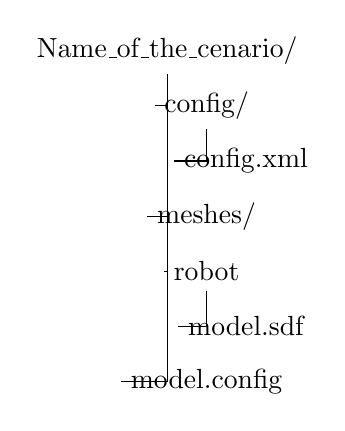
\begin{tikzpicture}[%
		grow via three points={one child at (0.5,-0.7) and
			two children at (0.5,-0.7) and (0.5,-1.4)},
		edge from parent path={(\tikzparentnode.south) |- (\tikzchildnode.west)}]
		\node {Name\_of\_the\_cenario/}
		child { node {config/}
			child { node {config.xml}}
		}
		child [missing] {}
		child { node {meshes/}}		
		child { node {robot}
			child { node {model.sdf}}
		}
		child [missing] {}
		child { node {model.config}};
		\end{tikzpicture}
		\caption{Scenarios directories organization. The directories are represented by the retangular shapes with ''/'' in the end. The files are represented by the retangular shapes with some extension type at the end.}
		\label{cenario1}
	\end{figure}
	
	\begin{itemize}
		\itemsep0em 
		\item[-]The ''config.xml'' file stores information from the control strategy used in the UAV simulation.
		\item[-]The ''meshes'' directory store the file responsable to generate the scenario visual representation.
		\item[-]The ''model.sdf'' file describes the scenario visual model to the \textit{Gazebo}.
		\item[-]The ''model.config'' file describes the model metadata.
	\end{itemize}
	
	The second part is the ".world" file configuration where the UAV used in the simulation is defined as well as the scenario associated with it. To access the directories and files bellow the user should type the directory \textit{Worlds} path in a shell terminal: 
	
	\begin{bashcode}
		$HOME/catkin_ws/src/ProVANT-Simulator/source/Database/worlds/worlds
		\end{bashcode}
		
		\begin{figure}[H]
			\center
			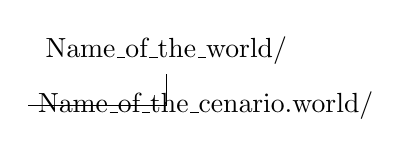
\begin{tikzpicture}[%
			grow via three points={one child at (0.5,-0.7) and
				two children at (0.5,-0.7) and (0.5,-1.4)},
			edge from parent path={(\tikzparentnode.south) |- (\tikzchildnode.west)}]
			\node {Name\_of\_the\_world/}
			child { node {Name\_of\_the\_cenario.world/}
			};
			\end{tikzpicture}
			\caption{Scenarios directories organization. The directories are represented by the retangular shapes with ''/'' in the end. The files are represented by the retangular shapes with some extension type at the end.}
			\label{cenario2}
		\end{figure}
		
		\begin{itemize}
			\itemsep0em 
			\item[-]The ''.world'' file is where the UAV used in the simulation is defined as well as the scenario associated with it.
		\end{itemize}
		
		
		\section{Obtaining the Scenario}
		

		The scenarios are obtained downloading ".dae" files. The DAE(Digital Asset Exchange files) extension is used to transfer images, textures and 3D models betweend graphical programs. The files are based on COLLADA, which uses a XML based system to guarantee compatibility betweend different graphical tools. This files can be downloaded at: \url{https://3dwarehouse.sketchup.com/}
		

		
		\begin{figure*}[!ht]
			\centering
			\includegraphics[width=450pt]{figuras/3dwh.png}
			\caption{3dwarehouse website}
			\label{3dwh}
		\end{figure*}
		
		Once the scenario has been choosed, the user should download the file as a COLLADA file as shown in \ref{ny} and then save the files at the \textit{meshes} directory explicited in \ref{cenario1}.
		
		
		\begin{figure*}[!ht]
			\centering
			\includegraphics[width=350pt]{figuras/ny.png}
			\caption{Cenário}
			\label{ny}
		\end{figure*}
		
		
		\begin{figure*}[!ht]
			\centering
			\includegraphics[width=150pt]{figuras/modelinfo.png}
			\caption{Numero de \textit{Polygons}}
			\label{modelinfo}
		\end{figure*}
		
		Some information have to be analysed from the 3dwarehouse website. In the \textit{model info} section of figure \ref{modelinfo} is possible to note the \textit{Polygon} parameter. A polygonal mesh is a collection of vertices, edges and faces that define the form of a 3D object. A high count of \textit{Polygons} demands vastly from the GPU and can slow down the simulation. 
		
		In order to avoid such problem the user must choose a scenario with a low \textit{Polygon} count or use a \textit{mesh modifier} to reduce the \textit{Polygon} count. The second option shall be treated in the next section.

		
		
		\section{Treating the Scenario}
		
		To decrease the number of \textit{Polygon} count the use of a \textit{mesh modifier} is necessary, in this case, Blender's \textit{Decimate Modiifer} is the \textit{mesh modifier} chosen. The first step is to download Blender.
		Once Blender is installed, the ".dae" file from the \textit{meshes} directory should be imported. Then, in the right corner menu the user should select the mesh modifier.
			
			\begin{figure*}[!ht]
			\centering
			\includegraphics[width=250pt]{figuras/decimod.png}
			\caption{\textit{Decimate Modifier}}
			\label{decimod}
			\end{figure*}
		
		There are three available options for simplifying the mesh: \textit{Collapse},\textit{Un-subdivide} and \textit{Planar}.
		\begin{itemize}
			\item \textbf{\textit{Collapse}}:
			
			Progressively unites the vertices taking in to account the mesh shape. There are four parameters in this modifier:
			\begin{itemize}
				\item [-] \textit{Ratio}: Define the collapsed vertices ratio. If the values is equal to 1, the mesh is not altered, if the value is 0.5 half of the faces are collapsed, and if the values equals to 0 all faces have been removed.
				\item [-] \textit{Factor}: The amount of influence the Vertex Group has on the decimation.
				\item [-] \textit{Triangulate}: Keeps any resulting triangulated geometry from the decimation process.
				\item [-] \textit{Symmetry}: Maintains symmetry on a single axis.
			\end{itemize}
		\begin{figure*}[!ht]
			\centering
			\includegraphics[width=200pt]{figuras/hillblendermod.png}
			\caption{\textit{\textit{Collapse}}}
			\label{collapse}
		\end{figure*}
		\item \textbf{\textit{Un-subdivide}}:It can be thought of as the reverse of subdivide. It attempts to remove edges that were the result of a subdivide operation. It is intended for meshes with a mainly grid-based topology (without giving uneven geometry). If additional editing has been done after the subdivide operation, the results may be unexpected.
		\begin{itemize}
			\item [-] \textit{Iterations}:The number of times to perform the un-subdivide operation. Two iterations is the same as one subdivide operation, so you will usually want to use even numbers.
		\end{itemize}
	\begin{figure*}[!ht]
		\centering
		\includegraphics[width=200pt]{figuras/unsubdiv.png}
		\caption{\textit{\textit{Un-subdivide}}}
		\label{unsubdiv}
	\end{figure*}
		\item \textbf{\textit{Planar}}:It reduces details on forms comprised of mainly flat surfaces.
		\begin{itemize}
			\item [-] \textit{Angle Limit}:Dissolve geometry which form angles (between surfaces) higher than this setting.
			\item [-] \textit{All Boundaries}: When enabled, all vertices along the boundaries of faces are dissolved. This can give nicer results when using a high Angle Limit.
			\item [-] \textit{Delimit}: Prevent dissolving geometry in certain places.
		\end{itemize}
		\begin{figure*}[!ht]
		\centering
		\includegraphics[width=200pt]{figuras/planar.png}
		\caption{\textit{\textit{Planar}}}
		\label{planar}
		\end{figure*}
		\end{itemize}
		
		At the top left menu the user should export the modified file with the ".dae" extension to the \textit{meshes} directory following the organization showned in \ref{cenario1}.

		
		
		\section{Scenario Configuration}
		
		Once the ".dae" file is treated is then necessary to start to configure the directories and files as showned in \ref{cenario1}

			\begin{bashcode}
			$HOME/catkin_ws/src/ProVANT-Simulator/source/Database/models/
			\end{bashcode}
		
	The user should configure the "model.sdf" file as visual link only as showned bellow.			

			
			\begin{minted}{xml}
	<model name="scenario_name">
		<pose>0 0 0  0 0 0</pose>
			<static>true</static>
				<link name="link_name">
				<visual name="scenario_visual_name">
				 <pose>0 0 0 0 0 0</pose>
				  <geometry>
					<mesh>
			<uri>model://scenario_directory_name/meshes/dae_file_name.dae</uri>
					</mesh>
				  </geometry>
				</visual>
			   </link>
			</model>
		</sdf>
		\end{minted}
		\centerline{Code: "model.sdf" description for a scenario}	
			
	    In the "meshes" directory the ".dae" files modified in blender as well as any texture file should be included. The "config.xml" file must be the same file from the uav the user intends to use with the scenario during the simulation.
		
		\begin{minted}{xml}
	
		<config>
	    <topicdata>data</topicdata>
		<TopicoStep>Step</TopicoStep>
		<Sampletime>12</Sampletime>
		<Strategy>Control_Strategy_of_Desired_UAV</Strategy>
		<RefPath>ref.txt</RefPath>
		<Outputfile>out.txt</Outputfile>
		<InputPath>in.txt</InputPath>
		<ErroPath>erro.txt</ErroPath>
		<Sensors>
			<Device>Topic_to_Receive_States_of_Desired_UAV</Device>
		</Sensors>
		<Actuators>
			<Device>Actuator_of_Desired_UAV</Device>
			.
			.
			.
			<Device>Actuator_of_Desired_UAV</Device>
		</Actuators>
		</config>
				\end{minted}
			\centerline{Code: "config.xml" description for a scenario}	
		
	\begin{itemize}
	\setlength{\itemsep}{1pt}
	\setlength{\parskip}{0pt}
	\setlength{\parsep}{0pt}
	\item[-] \textcolor{blue}{<Strategy></Strategy>}: especify the control strategy binary of the chosen uav;
	\item[-] \textcolor{blue}{<Sensors></Sensors>}: topic where the uav states are published;
	\item[-] \textcolor{blue}{<Actuators></Actuators>}: topics that receive the control signals and apply to the uav;
	\end{itemize} \normalsize
	
	The "model.config" file can be configures as showned:
	
	\begin{minted}{xml}
	<model>
		<name>scenario_name</name>
		<version>1.0</version>
		<sdf version="1.4">robot/model.sdf</sdf>
		<author>
			<name></name>
			<email></email>
		</author>
		<description></description>
	</model>
	\end{minted}
	\centerline{Code: "model.config" file description for a scenario}
	
	
		\begin{bashcode}
	$HOME/catkin_ws/src/ProVANT-Simulator/source/Database/worlds/worlds
\end{bashcode}
	The ".world" file must be configured as follows:	
	\begin{minted}{xml}
<world name="/HOME/catkin_ws/src/ProVANT-Simulator/source/Database/worlds/worlds
/scenario_world_directory/file_name.world">
	<gravity>0 0 -9.8</gravity>
	<physics type="ode">
		<max_step_size>0.001</max_step_size>
		<real_time_factor>0</real_time_factor>
	</physics>
	<plugin name="gazebo_tutorials" filename="libgazebo_ros_world_plugin.so">
		<ok>nothil</ok>
	</plugin>
	<include>
		<uri>model://sun</uri>
		<static>true</static>
	</include>
	<include>
		<uri>model://Desired_UAV</uri>
		<name>Arbitrary_name_to_appear_in_Gazebo</name>
		<static>false</static>
		<pose>0 0 0 0 0 0</pose>
	</include>
	<include>
		<uri>model://Desired_scenario_from_models_directory</uri>
		<name>Arbitrary_name_to_appear_in_Gazebo</name>
		<static>true</static>
		<pose>0 0 0 0 0 0</pose>
	</include>
	<scene>
		<sky>
			<time>18</time>
			<clouds>
			<speed>0</speed>
			</clouds>
		</sky>
	</scene>
</world>
</sdf>
	\end{minted}
	\centerline{Code: ".world" file description for a scenario}	
	
	\section{Example}
		\subsection{UAV 4.0 Scenario}
		
	The first step is to download the file and using the option \textit{import} in the top menu \textit{File} tab on Blender open the ".dae" file as showned in \ref{hillblender} 	
		

	\begin{figure*}[!ht]
	\centering
	\includegraphics[width=350pt]{figuras/hillblender.png}
	\caption{Scenario in Blender}
	\label{hillblender}
\end{figure*}

	
	In the right menu of blender the user should select one of the three options presented in the \textit{modifiers} tab: \textit{Collapse}, \textit{Un-subdivide} or \textit{Planar}. In the application the option \textit{Collapse} was chosen so the vertices woulb progressively joined but keeping the mesh shape into account. In this case the parameter to b modified is the \textit{ratio} parameter, which defines the collapsed vertices ratio. As presentd in the sections above, a ratio value of 1 keeps the mesh unchanged. It's possible to follow the number of removed faces when using a \textit{modifier} by checking the \textit{faces} option shown in \ref{hillblendermod}. It's important that after the \textit{modifiers} are applied the user must select the \textit{Apply} option so the changes are saved.
	
	
		\begin{figure*}[!ht]
		\centering
		\includegraphics[width=250pt]{figuras/hillblendermod.png}
		\caption{\textit{Collapse} in 3D Blender}
		\label{hillblendermod}
	\end{figure*}
	
	Once the modifications are saved the user should export the model as a ".dae" file using the top left menu \textit{File} tab and selecting the \textit{export} option. Create the directories and files as showned in \ref{cenario1} and then save the ".dae" file in the \textit{meshes} directory of the scenario model. In this case, the file is on the path bellow:

	
	\begin{bashcode}
	$HOME/catkin_ws/srcProVANT-Simulator/source/Database/models/cenario_hill/meshes	
		\end{bashcode}
	\label{daefile}
	

At the \textit{meshes} directory, besides of the ".dae" file, the textures files should also be included as shown in \ref{mesheshill}



			\begin{figure*}[!ht]
	\centering
	\includegraphics[width=350pt]{figuras/mesheshill.png}
	\caption{\textit{meshes} Directory}
	\label{mesheshill}
\end{figure*}

The scenario "model.sdf" file must be configured then. To do so the user should head to the scenario model diretory and at the "robot" directory open the "model.sdf" file with the user's editor of preference.  
				\begin{bashcode}
	$HOME/catkin_ws/src/ProVANT-Simulator/source/Database/models/cenario_hill/robot	
\end{bashcode}

			\begin{figure*}[!ht]
	\centering
	\includegraphics[width=350pt]{figuras/excenario.png}
	\caption{Scenario "model.sdf" file example}
	\label{excenario}
	\end{figure*}

The scenario "model.sdf" file should only contain a link with visual properties as showned in \ref{excenario}. The "model.config" file must be configured as \ref{ex2cenario} with the appropriate description.



			\begin{figure*}[!ht]
	\centering
	\includegraphics[width=350pt]{figuras/ex2cenario.png}
	\caption{Scenario "model.config" file example}
	\label{ex2cenario}
\end{figure*}

Still at the scenario model directory the user should configure the 'config.xml" file. Definig UAV 4.0 (\ref{vant4}) as the simulation uav, both uav "config.xml" file and the scenario "config.xml" file should be the same. This is due the internal simulator software organization. The file is configured as shown in \ref{ex3cenario}.

			\begin{figure*}[!ht]
	\centering
	\includegraphics[width=200pt]{figuras/ex3cenario.png}
	\caption{Scenario "config.xml" example when using UAV 4.0.}
	\label{ex3cenario}
\end{figure*}

Then the user should create the directories and files as in \ref{cenario2}. In this example, the directory where the ".world" file is located is the Hill directory at the \ref{worldshill} path.


				\begin{bashcode}
	$HOME/catkin_ws/src/ProVANT-Simulator/source/Database/worlds/worlds/Hill	
	\end{bashcode}
\label{worldshill}

The ".world" file is configured as showned in figure \ref{ex4cenario}

			\begin{figure*}[!ht]
	\centering
	\includegraphics[width=350pt]{figuras/ex4cenario.png}
	\caption{".world" File configured for a scenario using UAV 4.0.}
	\label{ex4cenario}
\end{figure*}

It's important to understand the \textit{tags} that include both the UAV and the scenario model.
\begin{minted}{xml}
<include>
	<uri>model://vant_4_aerod</uri>
	<name>newmodel</name>
	<static>false</static>
	<pose>0 0 0 0 0 0</pose>
</include>
<include>
	<uri>model://cenario_hill</uri>
	<name>cenario_hill</name>
	<static>true</static>
	<pose>0 0 0 0 0 0</pose>
</include>
 \end{minted}
	\centerline{Code: Including UAV and scenario model in the ".world" file.}


\begin{itemize}
	\itemsep0em
	\item[-] <uri></uri>: Search for the UAV and scenario models in the \textit{model} directory.
	\item[-] <name></name>: UAV and Scenario names displayed in Gazebo.
	\item[-] <static></static>: Indicates if the object is static in the simulation.
	\item[-] <pose></pose>: For the uav, the pose should be the same as the pose for the uav without scenario, and for the scenario the pose should be the one displayed in the figured. 
\end{itemize}

Doing so the simulation will be ready to be launched. To start the UAV 4.0 with scenario simulation the user should follow the steps presented in section \ref{workflow} examples.

			\begin{figure*}[!ht]
	\centering
	\includegraphics[width=350pt]{figuras/exhill.png}
	\caption{UAV 4.0 with Scenario Simulation}
	\label{exhill}
\end{figure*}

\bibliography{refs}

\end{document}